\documentclass[10pt,a4paper,twocolumn]{article}

\usepackage[utf8]{inputenc}
\usepackage[T1]{fontenc}
\usepackage{lmodern}
\usepackage[margin=1.8cm]{geometry}
\usepackage{amsmath,amssymb,amsfonts}
\usepackage{booktabs}
\usepackage{tabularx}
\usepackage{multirow}
\usepackage{graphicx}
\usepackage{xcolor}
\usepackage[numbers,sort&compress]{natbib}
\usepackage[colorlinks=true,linkcolor=blue!70!black,citecolor=blue!70!black,urlcolor=blue!70!black]{hyperref}

\setlength{\columnsep}{0.65cm}

\title{\textbf{DeepMzyme: Multimodal 3D Equivariant Graph and Protein Language Model Fusion for Transition-Metal Identity Prediction in Protein Binding Sites}}

\author{
  \textbf{Gilad Mechtinger}$^{1,*}$ \\[4pt]
  \small $^1$Tel Aviv University, Tel Aviv, Israel \\
  \small $^*$Correspondence: \href{https://github.com/MECHTI1}{\texttt{@MECHTI1}}
}

\date{}

\begin{document}

\twocolumn[
  \begin{@twocolumnfalse}
    \maketitle
    \begin{abstract}
      \noindent\textbf{Motivation:} First-row transition metal ions ($\text{Mn}$, $\text{Fe}$, $\text{Co}$, $\text{Ni}$, $\text{Cu}$, and $\text{Zn}$) serve as indispensable catalytic and structural cofactors across roughly one-third of characterized proteins. However, experimental macromolecular structures in the Protein Data Bank frequently suffer from metal misassignment, crystallization-buffer substitution, or metal loss, while predicted structures from modern structure-prediction models lack explicit cofactors altogether. Existing machine-learning classifiers such as PinMyMetal rely on 93 handcrafted tabular descriptors derived from external coordination-chemistry programs, collapse iron, cobalt, and nickel into a single undifferentiated class (\texttt{Class VIII}), and were evaluated under ungrouped cross-validation splits.\\[4pt]
      \noindent\textbf{Results:} We present \textbf{DeepMzyme}, an end-to-end multimodal deep learning framework that integrates $SE(3)$-equivariant Geometric Vector Perceptron Graph Neural Networks (\texttt{GVP-GNN}) over $8.0\text{ \AA}$ 3D binding-site microenvironments with residue-level evolutionary representations from the 600-million-parameter \texttt{ESM-C} protein language model. To establish a rigorous, leak-free benchmark, we reconstructed \textbf{9,398 of 9,408 (99.89\%)} PinMyMetal benchmark metal sites directly as 3D coordinate structures, curated a symmetry-audited training cohort of \texttt{7,398} mononuclear ion sites grouped into \texttt{2,208} clusters at $\ge 90\%$ sequence identity, and uncovered an undocumented ground-truth bond-valence sum leak (\texttt{valence\_3a}) in PinMyMetal's released feature tables (\texttt{7,919/7,920} training rows and \texttt{1,488/1,488} test rows). In a pre-registered matched comparison on the exact same \texttt{7,398} training sites, $\ge 90\%$ sequence-identity 5-fold cross-validation splits, and \texttt{1,488} held-out test sites, DeepMzyme's pre-declared single model achieves \textbf{74.28\%} mean-fold (\textbf{74.34\%} pooled) balanced accuracy in cross-validation and \textbf{67.55\%} on the full reference test set (\textbf{69.33\%} on the \texttt{1,346} in-scope protein-coordinated sites), outperforming PinMyMetal's released classifier retrained with deployment-available features (\texttt{PMM-D}: \textbf{63.03\%} CV, \textbf{58.27\%} test) by \textbf{+11.25 percentage points (pp)} in cross-validation ($97.5\%$ CI $[+6.25, +15.36]$) and \textbf{+9.28 pp} on the test set ($97.5\%$ CI $[+3.59, +15.10]$). Across all 15 DeepMzyme ensembles selected strictly by cross-validation (and 6 seed-42-ranked CV ensembles), test balanced accuracy reaches \textbf{68.83\%--72.10\%} on the full test set (\textbf{70.49\%--73.64\%} on in-scope sites), outperforming \texttt{PMM-D} by \textbf{+10.56 to +13.83 pp} and outperforming PinMyMetal even when retaining the leaked \texttt{valence\_3a} feature (\texttt{PMM-R}: \textbf{67.19\%} CV, \textbf{63.41\%} test) by \textbf{+5.42 to +8.69 pp} (all paired $95\%$ CIs above zero). Furthermore, DeepMzyme provides the first homology-grouped cross-validation resolution within \texttt{Class VIII}, achieving \texttt{65.2\%} native 5-class balanced accuracy (\texttt{60.6\%} $\text{Fe}$ recall) and a \texttt{0.680} ($95\%$ CI $[0.582, 0.770]$) pairwise $\text{Co}$--$\text{Ni}$ AUROC.\\[4pt]
      \noindent\textbf{Availability and Implementation:} Source code, automated test suites, and evaluation pipelines are freely available at \url{https://github.com/MECHTI1/DeepMzyme}. The reconstructed 3D benchmark dataset (\texttt{9,398} sites, \texttt{1.1 GB}), structural bundles, and released checkpoints are hosted on Hugging Face at \url{https://huggingface.co/datasets/GMBioinformatics/DeepMzyme}.
    \end{abstract}
    \vspace{0.5cm}
  \end{@twocolumnfalse}
]

\section{Introduction}

Metalloproteins play central roles in biological catalysis, electron transfer, oxygen transport, and structural stabilization across all kingdoms of life. Between one-third and one-half of all structurally characterized enzymes require a bound metal cofactor for biological activity, with the late first-row transition metals---manganese ($\text{Mn}^{2+/3+}$), iron ($\text{Fe}^{2+/3+}$), cobalt ($\text{Co}^{2+/3+}$), nickel ($\text{Ni}^{2+}$), copper ($\text{Cu}^{+/2+}$), and zinc ($\text{Zn}^{2+}$)---mediating the vast majority of redox and hydrolytic reactions \cite{irving1953stability,zheng2017checkmymetal}. Despite their distinct chemical reactivities, accurately assigning the identity of a transition metal at a protein binding site in three-dimensional (3D) macromolecular structures remains a persistent challenge in structural bioinformatics.

Three biophysical and experimental factors underlie this difficulty. First, adjacent first-row transition-metal cations possess nearly identical ionic radii ($0.65\text{--}0.83\text{ \AA}$ in octahedral coordination) and similar electron counts ($Z = 25\text{--}30$), making them difficult to distinguish solely from conventional X-ray diffraction electron-density maps at moderate resolution in the absence of anomalous scattering experiments \cite{zheng2017checkmymetal}. Second, protein purification and heterologous expression frequently replace native cofactors with non-physiological metals abundant in expression media or crystallization buffers (most commonly $\text{Zn}^{2+}$ or $\text{Ni}^{2+}$), resulting in widespread metal misannotation in the Protein Data Bank (PDB). Third, as formalized by the Irving--Williams stability series ($\text{Mn}^{2+} < \text{Fe}^{2+} < \text{Co}^{2+} < \text{Ni}^{2+} < \text{Cu}^{2+} > \text{Zn}^{2+}$) \cite{irving1953stability}, first-shell protein ligands---predominantly the side chains of histidine ($\text{His}$), cysteine ($\text{Cys}$), aspartate ($\text{Asp}$), and glutamate ($\text{Glu}$)---are heavily shared across different transition metals. Consequently, metalloproteins achieve physiological metal selectivity not merely through first-shell donor identity, but through subtle second-shell hydrogen-bonding networks, steric constraints, electrostatic tuning, and long-range evolutionary sequence adaptations. With proteome-scale structure prediction methods such as AlphaFold2 \cite{jumper2021alphafold}, AlphaFold3 \cite{abramson2024alphafold3}, and ESMFold \cite{lin2023esmfold} generating millions of protein models that either lack cofactors or require post-hoc cofactor assignment, computational frameworks capable of inferring transition-metal identity directly from 3D pocket coordinates and protein sequence are essential.

Early computational approaches to metalloprotein characterization relied on geometric templates, bond-valence sum (BVS) calculations (e.g., CheckMyMetal \cite{zheng2017checkmymetal}), or random-forest classifiers trained on physicochemical pocket descriptors (e.g., MAHOMES \cite{feehan2021mahomes}). More recently, deep learning methods have addressed metal-site localization and classification. Metal3D \cite{durr2023metal3d} introduced voxelized 3D convolutional neural networks trained on zinc-binding sites to predict continuous spatial metal density, achieving high spatial localization precision without predicting metal element identity. AllMetal3D \cite{durr2025allmetal3d} extended voxelized representations to multi-class ion identity prediction, but reported approximately $46\%$ overall accuracy across 12 metal ions and noted that static local geometry alone struggles to separate physicochemically similar transition metals.

Recently, Zhang \textit{et al.} \cite{zhang2025pinmymetal} introduced \textbf{PinMyMetal (PMM)} in \textit{Nature Communications}, a two-stage pipeline combining binding-site localization with a five-estimator soft-voting classifier (Logistic Regression, Balanced Random Forest, Multi-Layer Perceptron, Support Vector Classifier, and EasyEnsemble) trained on 93 handcrafted tabular features extracted via the \texttt{NEIGHBORHOOD} database program and bond-valence tables. PinMyMetal formulated transition-metal classification over four classes---$\text{Mn}$, $\text{Cu}$, $\text{Zn}$, and $\text{Class VIII}$ ($\text{Fe} + \text{Co} + \text{Ni}$)---reporting $75.08\%$ 5-fold cross-validation macro-precision ($\approx 72.70\%$ balanced accuracy) and $67.85\%$ balanced accuracy on a \texttt{1,488}-site held-out test set.

However, a rigorous forensic examination of the released PinMyMetal benchmark and evaluation protocol reveals four fundamental limitations that confound both its reported performance and its applicability to end-to-end 3D deep learning:
\begin{enumerate}
  \item \textbf{Absence of Public Ion-Level 3D Coordinates:} PinMyMetal's released training (\texttt{7,920} rows) and test (\texttt{1,488} rows) tables provide only precomputed numerical feature columns indexed by internal \texttt{NEIGHBORHOOD} database keys (\texttt{residueid\_ion}) rather than physical PDB chain and residue coordinates.
  \item \textbf{Ground-Truth Bond-Valence Label Leakage (\texttt{valence\_3a}):} While PinMyMetal's deployment code writes candidate sites as $\text{Zn}$ before invoking \texttt{NEIGHBORHOOD}---so that generic $3\text{ \AA}$ and $4\text{ \AA}$ bond-valence features (\texttt{valence\_3a}, \texttt{valence\_4a}, \texttt{vecsum\_3a}, \texttt{vecsum\_4a}) equal their $\text{Zn}$-probe counterparts---the released training and test CSV tables were populated directly from native PDB structures where the ground-truth metal atom was already present. Consequently, in \texttt{7,919/7,920} (\texttt{99.99\%}) training rows and \texttt{1,488/1,488} (\texttt{100\%}) test rows, \texttt{valence\_3a} equals the bond-valence sum computed under the \textbf{true ground-truth metal's oxidation state} (\texttt{bvs\_mn}, \texttt{bvs\_fe}, \texttt{bvs\_co}, \texttt{bvs\_ni}, \texttt{bvs\_cu}, or \texttt{bvs\_zn}). A zero-parameter lookup comparing \texttt{valence\_3a} against the elemental \texttt{bvs\_*} columns recovers the true four-class label with \textbf{99.94\%--100\% balanced accuracy} on the training table.
  \item \textbf{Ungrouped Cross-Validation and Train--Test Homology Overlap:} PinMyMetal's published 5-fold cross-validation used ungrouped \texttt{StratifiedKFold(n\_splits=5, shuffle=False)} over raw CSV row order, allowing identical PDB entries, homologous chains, and \texttt{503} crystallographic symmetry-linked ions to span training and validation splits. Moreover, \texttt{809} of the \texttt{1,488} test rows (\texttt{54.4\%}, spanning \texttt{668} shared PDB IDs) come from PDB entries also present in the training set.
  \item \textbf{Coarse \texttt{Class VIII} Grouping:} By collapsing $\text{Fe}$, $\text{Co}$, and $\text{Ni}$ into a single target class, PinMyMetal cannot distinguish iron-dependent enzymes from cobalt- or nickel-dependent enzymes.
\end{enumerate}

In this work, we address each of these challenges by developing \textbf{DeepMzyme}, a bimodal geometric and evolutionary deep learning framework for metalloprotein binding sites. Our contributions are fourfold:
\begin{itemize}
  \item \textbf{Open 3D Benchmark Reconstruction \& Homology-Grouped Curation:} We reverse-engineered PinMyMetal's internal database keys via deterministic \texttt{NEIGHBORHOOD} coordinate crosswalks, recovering \textbf{9,398 of 9,408 (99.89\%)} benchmark ions as 3D structure files (\texttt{1.1 GB} public dataset), and established a symmetry-audited cohort of \texttt{7,398} mononuclear sites partitioned into 5 folds grouped at $\ge 90\%$ sequence identity (\texttt{2,208} clusters).
  \item \textbf{Multimodal $SE(3)$-Equivariant + Protein Language Model Architecture:} DeepMzyme fuses scalar and $SE(3)$-equivariant vector message passing (\texttt{GVP-GNN}) \cite{jing2021gvp} over $8.0\text{ \AA}$ 3D structural pocket graphs with full-chain \texttt{ESM-C 600M} \cite{esmc2024} residue embeddings, learning end-to-end from 3D coordinates and protein sequences without handcrafted \texttt{NEIGHBORHOOD} or bond-valence tables.
  \item \textbf{Pre-Registered Matched Superiority Over PinMyMetal:} Evaluated on identical training sites, $\ge 90\%$ sequence-identity folds, and test sets, DeepMzyme outperforms PinMyMetal's classifier retrained with deployment-available features (\texttt{PMM-D}) by \textbf{+11.25 pp} in 5-fold CV and \textbf{+9.28 to +13.83 pp} on the held-out test set, and outperforms PinMyMetal even when retaining the leaked \texttt{valence\_3a} feature (\texttt{PMM-R}) by \textbf{+5.42 to +8.69 pp} across all CV-selected ensembles.
  \item \textbf{Sub-\texttt{Class VIII} Resolution and Multimodal Optimization Insights:} We demonstrate how differential trunk-versus-head learning rates (\texttt{1e-4} vs.\ \texttt{3e-4}) prevent 3D GNN overfitting in multimodal fusion (\texttt{+3.12 pp} over sequence-only and \texttt{+2.20 pp} over $L_2$-tuned structure-only baselines), and provide the first homology-grouped 5-class ($\text{Fe}$ vs.\ $\text{Co+Ni}$) and 6-class ($\text{Fe}$, $\text{Co}$, $\text{Ni}$) transition-metal resolution.
\end{itemize}

\section{Materials and Methods}

\subsection{Ion-Level 3D Reconstruction of the PinMyMetal Benchmark}

PinMyMetal's released benchmark tables (\texttt{classmodel\_train\_set} containing \texttt{7,920} rows across \texttt{4,195} PDB IDs and \texttt{classmodel\_test\_set} containing \texttt{1,488} rows across \texttt{1,179} PDB IDs) identify each metal-binding site solely by \texttt{(pdbid, residueid\_ion, metalid)}, where \texttt{residueid\_ion} is an internal sequential integer generated at runtime by the compiled C/Fortran \texttt{NEIGHBORHOOD} program. Because \texttt{residueid\_ion} does not correspond to standard PDB residue sequence numbers (\texttt{resseq}) or chain identifiers, 3D coordinates cannot be trivially indexed from the CSV tables alone.

To reconstruct the exact 3D atomic coordinates of every benchmark site, we executed the \texttt{neighborhood} binary distributed in \texttt{PinMyMetal\_V1.0\_zenodo.zip} (\texttt{10.5281/zenodo.17610514}) across all source PDB depositions and parsed the resulting relational \texttt{.data} tables (\texttt{atoms.data}, \texttt{residues.data}, and \texttt{neighbors.data}) to establish a deterministic crosswalk mapping \texttt{(pdbid, residueid\_ion, metalid)} to physical PDB coordinates \texttt{(chain\_id, resseq, icode, resname, atom\_name, x, y, z)}. For \texttt{298} large macromolecular assemblies where the legacy \texttt{neighborhood} binary terminated with a segmentation fault (\texttt{SIGSEGV}) due to fixed internal atom-table buffer limits, stripping non-coordinating crystallographic water (\texttt{HOH}) records prior to execution resolved all buffer overflows and recovered 100\% of the affected sites with bit-identical protein-ligand topology. In total, \textbf{9,398 of 9,408 (99.89\%)} benchmark ions---comprising \textbf{7,911 of 7,920 (99.89\%)} training rows and \textbf{1,487 of 1,488 (99.93\%)} test rows across \texttt{7,724} structure files---were exactly recovered and released on Hugging Face (\texttt{GMBioinformatics/DeepMzyme}).

\subsection{Forensic Audit of the \texttt{valence\_3a} Bond-Valence Leak (\texttt{TECH-028})}

During feature-table verification, we audited all 93 feature columns in PinMyMetal's released training and test CSVs against PinMyMetal's open-source inference pipeline (\texttt{PinMyMetal.py} and \texttt{generate\_features.py}). In PinMyMetal's deployment pipeline, candidate metal sites predicted by the localization module have unknown element identity and are written to a temporary PDB file as zinc (\texttt{ZN}) before running \texttt{NEIGHBORHOOD}. Under that deployment protocol, the ten elemental bond-valence columns (\texttt{bvs\_mn}, \texttt{bvs\_fe}, \texttt{bvs\_co}, \texttt{bvs\_ni}, \texttt{bvs\_cu}, \texttt{bvs\_zn} at $3\text{ \AA}$, and \texttt{bvs\_4a\_*} at $4\text{ \AA}$) are computed using element-specific bond-valence parameters $R_0$, while the four generic summary columns (\texttt{valence\_3a}, \texttt{valence\_4a}, \texttt{vecsum\_3a}, \texttt{vecsum\_4a}) are computed by \texttt{NEIGHBORHOOD} using the atom name written in the PDB file---which at deployment is always $\text{Zn}$, making $\texttt{valence\_3a} = \texttt{bvs\_zn}$.

In contrast, PinMyMetal's released training (\texttt{7,920} rows) and test (\texttt{1,488} rows) tables were generated by running \texttt{NEIGHBORHOOD} on experimental PDB files containing the \textbf{ground-truth metal ion labels}. Consequently, in \texttt{7,919 of 7,920} (\texttt{99.99\%}) training rows and \texttt{1,488 of 1,488} (\texttt{100\%}) test rows, \texttt{valence\_3a} is not equal to \texttt{bvs\_zn}, but instead equals the elemental bond-valence sum \texttt{bvs\_<true\_metal>} of the site's ground-truth metal label (within floating-point rounding $\le 10^{-3}$). Because the six elemental \texttt{bvs\_*} columns are simultaneously present in the same feature vector, any nonlinear classifier or decision tree can compare \texttt{valence\_3a} against $(\texttt{bvs\_mn}, \texttt{bvs\_fe}, \texttt{bvs\_co}, \texttt{bvs\_ni}, \texttt{bvs\_cu}, \texttt{bvs\_zn})$ to read off the true metal identity. Indeed, a parameter-free rule assigning each row to the class whose \texttt{bvs\_*} column matches \texttt{valence\_3a} achieves \textbf{99.94\%--100\% four-class balanced accuracy} on \texttt{classmodel\_train\_set}. To separate true generalization from this target-leakage artifact, our matched comparator experiments evaluate PinMyMetal both with deployment-available features (\texttt{PMM-D}, 89 features omitting \texttt{valence\_3a/4a} and \texttt{vecsum\_3a/4a}) and with all 93 released features (\texttt{PMM-R}).

\subsection{Curating the \texttt{7,398}-Ion Training Cohort and $\ge 90\%$ Sequence-Identity Folds}

Auditing the \texttt{7,920} source training rows identified \texttt{522} rows that violate mononuclear protein-pocket assumptions:
\begin{itemize}
  \item \textbf{9 rows} absent from source PDB coordinate recovery;
  \item \textbf{10 rows} mapping to polynuclear clusters or non-single-metal species (e.g., $\text{Fe--S}$ iron--sulfur clusters or \texttt{UNX} unknown ligand records); and
  \item \textbf{503 rows} flagged with explicit crystallographic symmetry \texttt{LINK} records between the target metal ion and symmetry-related protein chains across unit-cell boundaries, where standard asymmetric-unit coordinates truncate first-shell protein ligands.
\end{itemize}
Excluding these \texttt{522} rows produced the certified \textbf{7,398-ion training cohort} (\texttt{SHA-256: 745b19c1644ee...}) spanning \texttt{3,992} unique PDB entries. Native element counts across the \texttt{7,398} sites are: \textbf{Mn:} \texttt{2,528} (\texttt{34.17\%}), \textbf{Zn:} \texttt{2,032} (\texttt{27.47\%}), \textbf{Class VIII:} \texttt{2,495} (\texttt{33.73\%})---comprising \textbf{Fe:} \texttt{1,737} (\texttt{23.48\%}), \textbf{Ni:} \texttt{475} (\texttt{6.42\%}), and \textbf{Co:} \texttt{283} (\texttt{3.83\%})---and \textbf{Cu:} \texttt{343} (\texttt{4.64\%}).

To prevent homologous data leakage during cross-validation, all protein chains associated with the \texttt{7,398} sites were clustered at $\ge 90\%$ sequence identity into \textbf{2,208 connected near-copy groups} (\texttt{v3-seqid90-s42-b2}). These \texttt{2,208} sequence-identity groups were partitioned into 5 stratified folds such that all sites sharing a PDB entry or belonging to chains with $\ge 90\%$ sequence identity reside strictly within the same fold.

\subsection{Reference Test Set Stratification (\texttt{1,488} Sites)}

PinMyMetal's \texttt{1,488}-site reference test set (\texttt{1,179} PDB entries; $\text{Mn}: 167$, $\text{Class VIII}: 252$, $\text{Cu}: 64$, $\text{Zn}: 1,005$ [\texttt{67.5\%}]) contains both crystallographic symmetry-linked ions and PDB entries that overlap with \texttt{classmodel\_train\_set}. Rather than altering the upstream test set, we evaluate all models across five nested, pre-declared test subsets:
\begin{enumerate}
  \item \textbf{Full Reference Test (\texttt{1,488} rows, \texttt{1,179} PDB entries):} Evaluates all \texttt{1,488} rows in \texttt{classmodel\_test\_set}. The \texttt{3} unscorable rows (1 missing structure \texttt{8c4y}, 2 empty protein graphs) are scored as unconditional errors (\texttt{0} credit) for DeepMzyme.
  \item \textbf{LINK-Free Subset (\texttt{1,349} rows):} Excludes \texttt{139} test rows carrying crystallographic symmetry \texttt{LINK} flags.
  \item \textbf{In-Scope / Training-Eligible Subset (\texttt{1,346} rows, \texttt{1,093} PDB entries):} Scored, LINK-free primary sites that satisfy the biological scope filter ($\ge 1$ coordinating protein donor atom within the binding site, excluding water-only or nucleic-acid-only buffer ions).
  \item \textbf{Deduplicated Subset (\texttt{1,098} rows):} Retains one representative site per near-identical structure group within the test set.
  \item \textbf{Homology-Filtered Clean Subset (\texttt{423} rows, \texttt{352} PDB entries):} Excludes all \texttt{809} test rows that share a PDB ID with the training set (\texttt{668} shared PDB IDs) as well as all test chains sharing $\ge 90\%$ sequence identity or homology with training chains.
\end{enumerate}

\subsection{DeepMzyme Multimodal Architecture (\texttt{GVP-GNN + ESM-C 600M})}

DeepMzyme models each metal-binding microenvironment as a bimodal learning problem combining a local 3D $SE(3)$-equivariant pocket graph encoder with a full-chain evolutionary sequence encoder.

\paragraph{1. 3D Equivariant Pocket Graph Branch (\texttt{GVP-GNN}).}
For a target metal site at coordinate $\mathbf{x}_M \in \mathbb{R}^3$, we construct a spatial radius graph $\mathcal{G} = (\mathcal{V}, \mathcal{E})$ comprising all protein residues $i \in \mathcal{V}$ whose $\text{C}_\alpha$ atom (or coordinating side-chain donor atom) lies within $r_{\text{pocket}} = 8.0\text{ \AA}$ of $\mathbf{x}_M$. Notice that the metal ion's chemical identity is never provided as an input feature. Each residue node $i \in \mathcal{V}$ is endowed with a tuple of scalar features $\mathbf{s}_i \in \mathbb{R}^{d_s}$ and $SE(3)$-equivariant vector features $\mathbf{V}_i \in \mathbb{R}^{\nu_n \times 3}$:
\begin{itemize}
  \item \textbf{Node Scalar Features ($\mathbf{s}_i$):} A 20-dimensional one-hot amino-acid encoding, continuous residue physicochemical descriptors, explicit first-shell ($\le 3.0\text{ \AA}$) and second-shell ($\le 5.0\text{ \AA}$) coordination role indicators, and 16-dimensional Gaussian radial basis function (RBF) encodings of the Euclidean distance $\|\mathbf{x}_i - \mathbf{x}_M\|_2$ to the metal center (with standardized raw distance channels). Optional \texttt{PROPKA} electrostatic $\Delta\text{p}K_a$ shifts \cite{olsson2011propka3} are also supported.
  \item \textbf{Node Vector Features ($\mathbf{V}_i$):} Unit direction vectors capturing side-chain orientation and radial orientation toward the metal site:
  \begin{equation}
    \mathbf{v}_i^{(1)} = \frac{\mathbf{x}_{\text{C}_\beta, i} - \mathbf{x}_{\text{C}_\alpha, i}}{\|\mathbf{x}_{\text{C}_\beta, i} - \mathbf{x}_{\text{C}_\alpha, i}\|_2 + \epsilon}, \quad
    \mathbf{v}_i^{(2)} = \frac{\mathbf{x}_M - \mathbf{x}_{\text{C}_\alpha, i}}{\|\mathbf{x}_M - \mathbf{x}_{\text{C}_\alpha, i}\|_2 + \epsilon}
  \end{equation}
  \item \textbf{Edge Features ($\mathbf{s}_{ij}, \mathbf{V}_{ij}$):} Directed edges $(j \to i) \in \mathcal{E}$ connect all residue pairs within $r_{\text{edge}} = 8.0\text{ \AA}$, carrying 16-dimensional Gaussian RBF distance encodings $\mathbf{s}_{ij} = \text{RBF}(\|\mathbf{x}_{\text{C}_\alpha, i} - \mathbf{x}_{\text{C}_\alpha, j}\|_2)$ and unit displacement vectors $\mathbf{V}_{ij} = (\mathbf{x}_{\text{C}_\alpha, j} - \mathbf{x}_{\text{C}_\alpha, i}) / (\|\mathbf{x}_{\text{C}_\alpha, j} - \mathbf{x}_{\text{C}_\alpha, i}\|_2 + \epsilon)$. Optional non-covalent residue interaction network (\texttt{RING}) edges \cite{clementel2022ring3} are also supported.
\end{itemize}

Node and edge representations are updated across $L_{\text{GVP}} = 3$ stacked Geometric Vector Perceptron (\texttt{GVP}) message-passing layers \cite{jing2021gvp}. Within each GVP layer, linear projections of vector channels are coupled with norms feeding into scalar gates, ensuring that scalar outputs remain strictly $SE(3)$-invariant while vector outputs transform equivariantly under 3D rotations $R \in SO(3)$:
\begin{equation}
  \text{GVP}\big((\mathbf{s}, \mathbf{V})\big) = \Big(\sigma\big(\mathbf{W}_s [\mathbf{s} \,\|\, \|\mathbf{W}_h \mathbf{V}\|_2] + \mathbf{b}_s\big),\; \sigma_g\big(\|\mathbf{W}_\mu \mathbf{W}_h \mathbf{V}\|_2\big) \odot (\mathbf{W}_\mu \mathbf{W}_h \mathbf{V})\Big)
\end{equation}
After message passing, equivariant vector channels are contracted into invariant scalars and aggregated across pocket nodes via mean and attention pooling to yield the 3D structural pocket representation $\mathbf{h}_{\text{GVP}} \in \mathbb{R}^{d_g}$.

\paragraph{2. Evolutionary Sequence Context Branch (\texttt{ESM-C 600M}).}
Because local pocket geometry within an $8.0\text{ \AA}$ sphere does not capture global fold family or long-range evolutionary constraints, the full-length amino-acid sequence of size $L$ for each coordinating protein chain is embedded using the frozen 600-million-parameter \textbf{ESM Cambrian (\texttt{esmc\_600m})} protein language model \cite{esmc2024}, producing contextualized per-residue representations $\mathbf{E} \in \mathbb{R}^{L \times 1152}$. For the subset of sequence positions $\mathcal{V}_{\text{seq}} \subseteq \{1, \dots, L\}$ belonging to the 3D binding pocket, residue embeddings $\mathbf{e}_i \in \mathbb{R}^{1152}$ are projected through a regularized linear + LayerNorm bottleneck ($\mathbb{R}^{1152} \to \mathbb{R}^{d_e}$) and aggregated over the pocket via concatenated mean and learned attention pooling:
\begin{equation}
  \mathbf{h}_{\text{ESM}} = \left[ \frac{1}{|\mathcal{V}_{\text{seq}}|} \sum_{i \in \mathcal{V}_{\text{seq}}} \tilde{\mathbf{e}}_i \;\middle\|\; \sum_{i \in \mathcal{V}_{\text{seq}}} \alpha_i \tilde{\mathbf{e}}_i \right], \quad \alpha_i = \frac{\exp(\mathbf{w}_a^\top \tanh(\mathbf{W}_a \tilde{\mathbf{e}}_i))}{\sum_{k \in \mathcal{V}_{\text{seq}}} \exp(\mathbf{w}_a^\top \tanh(\mathbf{W}_a \tilde{\mathbf{e}}_k))}
\end{equation}

\paragraph{3. Late Multimodal Fusion and Classification Head.}
In the late-fusion architecture (\texttt{--fusion-mode late\_fusion}), the invariant 3D pocket representation $\mathbf{h}_{\text{GVP}}$ and the evolutionary pocket representation $\mathbf{h}_{\text{ESM}}$ are concatenated and passed through a multi-layer perceptron (MLP) classifier with dropout ($p = 0.2$) to produce class logits $\mathbf{z} = f_{\text{MLP}}([\mathbf{h}_{\text{GVP}} \,\|\, \mathbf{h}_{\text{ESM}}])$.

\subsection{Target Formulations, Loss Recipes, and Differential Trunk Optimization}

DeepMzyme supports three native supervision granularities:
\begin{enumerate}
  \item \textbf{Direct 4-Class (\texttt{four\_class}):} Directly predicts $\mathcal{Y}_4 = \{\text{Mn}, \text{Cu}, \text{Zn}, \text{Class VIII}\}$.
  \item \textbf{Native 5-Class (\texttt{five\_class}):} Separates iron from cobalt and nickel, predicting $\mathcal{Y}_5 = \{\text{Mn}, \text{Cu}, \text{Zn}, \text{Fe}, \text{Co+Ni}\}$. For evaluation on the canonical 4-class benchmark, predicted probabilities are summed prior to $\arg\max$:
  \begin{equation}
    P(\text{Class VIII}) = P(\text{Fe}) + P(\text{Co+Ni})
  \end{equation}
  \item \textbf{Native 6-Class (\texttt{six\_class}):} Predicts all six individual transition metals $\mathcal{Y}_6 = \{\text{Mn}, \text{Fe}, \text{Co}, \text{Ni}, \text{Cu}, \text{Zn}\}$, collapsing to 4 classes via $P(\text{Class VIII}) = P(\text{Fe}) + P(\text{Co}) + P(\text{Ni})$.
\end{enumerate}

Across these target formulations, we evaluated three class-weighted cross-entropy loss recipes over 50 cosine-annealed epochs (batch size 16, terminal epoch-50 checkpoint selection) using \texttt{AdamW} \cite{loshchilov2019adamw}:
\begin{itemize}
  \item \textbf{Recipe \texttt{B} (Baseline):} Inverse-frequency class-weighted cross-entropy with weight decay $\lambda = 10^{-4}$.
  \item \textbf{Recipe \texttt{P} (Population-Normalized CE):} Population-normalized class weights designed to protect minority $\text{Cu}$ and sub-\texttt{Class VIII} recalls.
  \item \textbf{Recipe \texttt{S} (Label Smoothing):} Class-weighted cross-entropy with label smoothing $\varepsilon = 0.1$.
  \item \textbf{Differential Trunk Learning Rate (\texttt{trunklr1e4}):} In baseline multimodal runs, the randomly initialized 3D \texttt{GVP-GNN} trunk was trained at $\eta_{\text{GVP}} = 3 \times 10^{-4}$ while the \texttt{ESM-C} projection and fusion head used $\eta_{\text{head}} = 3 \times 10^{-5}$. To prevent the 3D GNN trunk from overfitting local pocket geometry faster than the sequence fusion layers converge, \texttt{trunklr1e4} lowers the GVP trunk learning rate to $\eta_{\text{GVP}} = 10^{-4}$.
\end{itemize}

\subsection{Matched PinMyMetal Retraining and Statistical Protocol}

To compare DeepMzyme and PinMyMetal under identical conditions, PinMyMetal's exact released 5-estimator soft-voting ensemble (\texttt{LogisticRegression + BalancedRandomForestClassifier + MLPClassifier + SVC + EasyEnsembleClassifier} with all published hyperparameters) was retrained in its pinned environment (\texttt{Python 3.11.5}, \texttt{scikit-learn 1.3.0}, \texttt{imbalanced-learn 0.11.0}) on the exact same \texttt{7,398} training sites and \texttt{v3-seqid90-s42-b2} 5-fold splits, and refit on all \texttt{7,398} sites to score the \texttt{1,488} test rows:
\begin{itemize}
  \item \textbf{\texttt{PMM-D} (Deployment-Faithful Comparator, 89 features):} Removes the 4 target-dependent columns (\texttt{valence\_3a}, \texttt{valence\_4a}, \texttt{vecsum\_3a}, \texttt{vecsum\_4a}).
  \item \textbf{\texttt{PMM-R} (Full Released-Table Comparator, 93 features):} Retains all 93 published columns including the leaked \texttt{valence\_3a} feature.
  \item \textbf{\texttt{PMM-D2} (Sensitivity Comparator, 79 features):} Removes both the 4 \texttt{valence/vecsum} columns and the 10 elemental \texttt{bvs\_*} columns.
  \item \textbf{\texttt{PMM-H} (Internal Tabular Feature Ablation, 89 features):} An untuned \texttt{HistGradientBoostingClassifier} trained on PinMyMetal's 89 deployment features to decouple tabular feature quality from PinMyMetal's released classifier architecture.
\end{itemize}

Primary performance is measured using unweighted four-class \textbf{balanced accuracy} (macro-averaged recall across $\text{Mn}$, $\text{Cu}$, $\text{Zn}$, and $\text{Class VIII}$):
\begin{equation}
  \text{BA} = \frac{1}{4} \sum_{c \in \{\text{Mn, Cu, Zn, VIII}\}} \frac{\text{TP}_c}{\text{TP}_c + \text{FN}_c}
\end{equation}
Alongside balanced accuracy, we report column-normalized \textbf{macro-precision} ($\frac{1}{4}\sum_c \frac{\text{TP}_c}{\text{TP}_c + \text{FP}_c}$), which is the metric printed on the diagonal of PinMyMetal's published Fig.\ 2a confusion matrix (\texttt{75.08\%}). Paired differences are evaluated via 10,000-replicate non-parametric cluster bootstrap resampling over PDB / sequence-identity groups.

\begin{figure*}[t!]
  \centering
  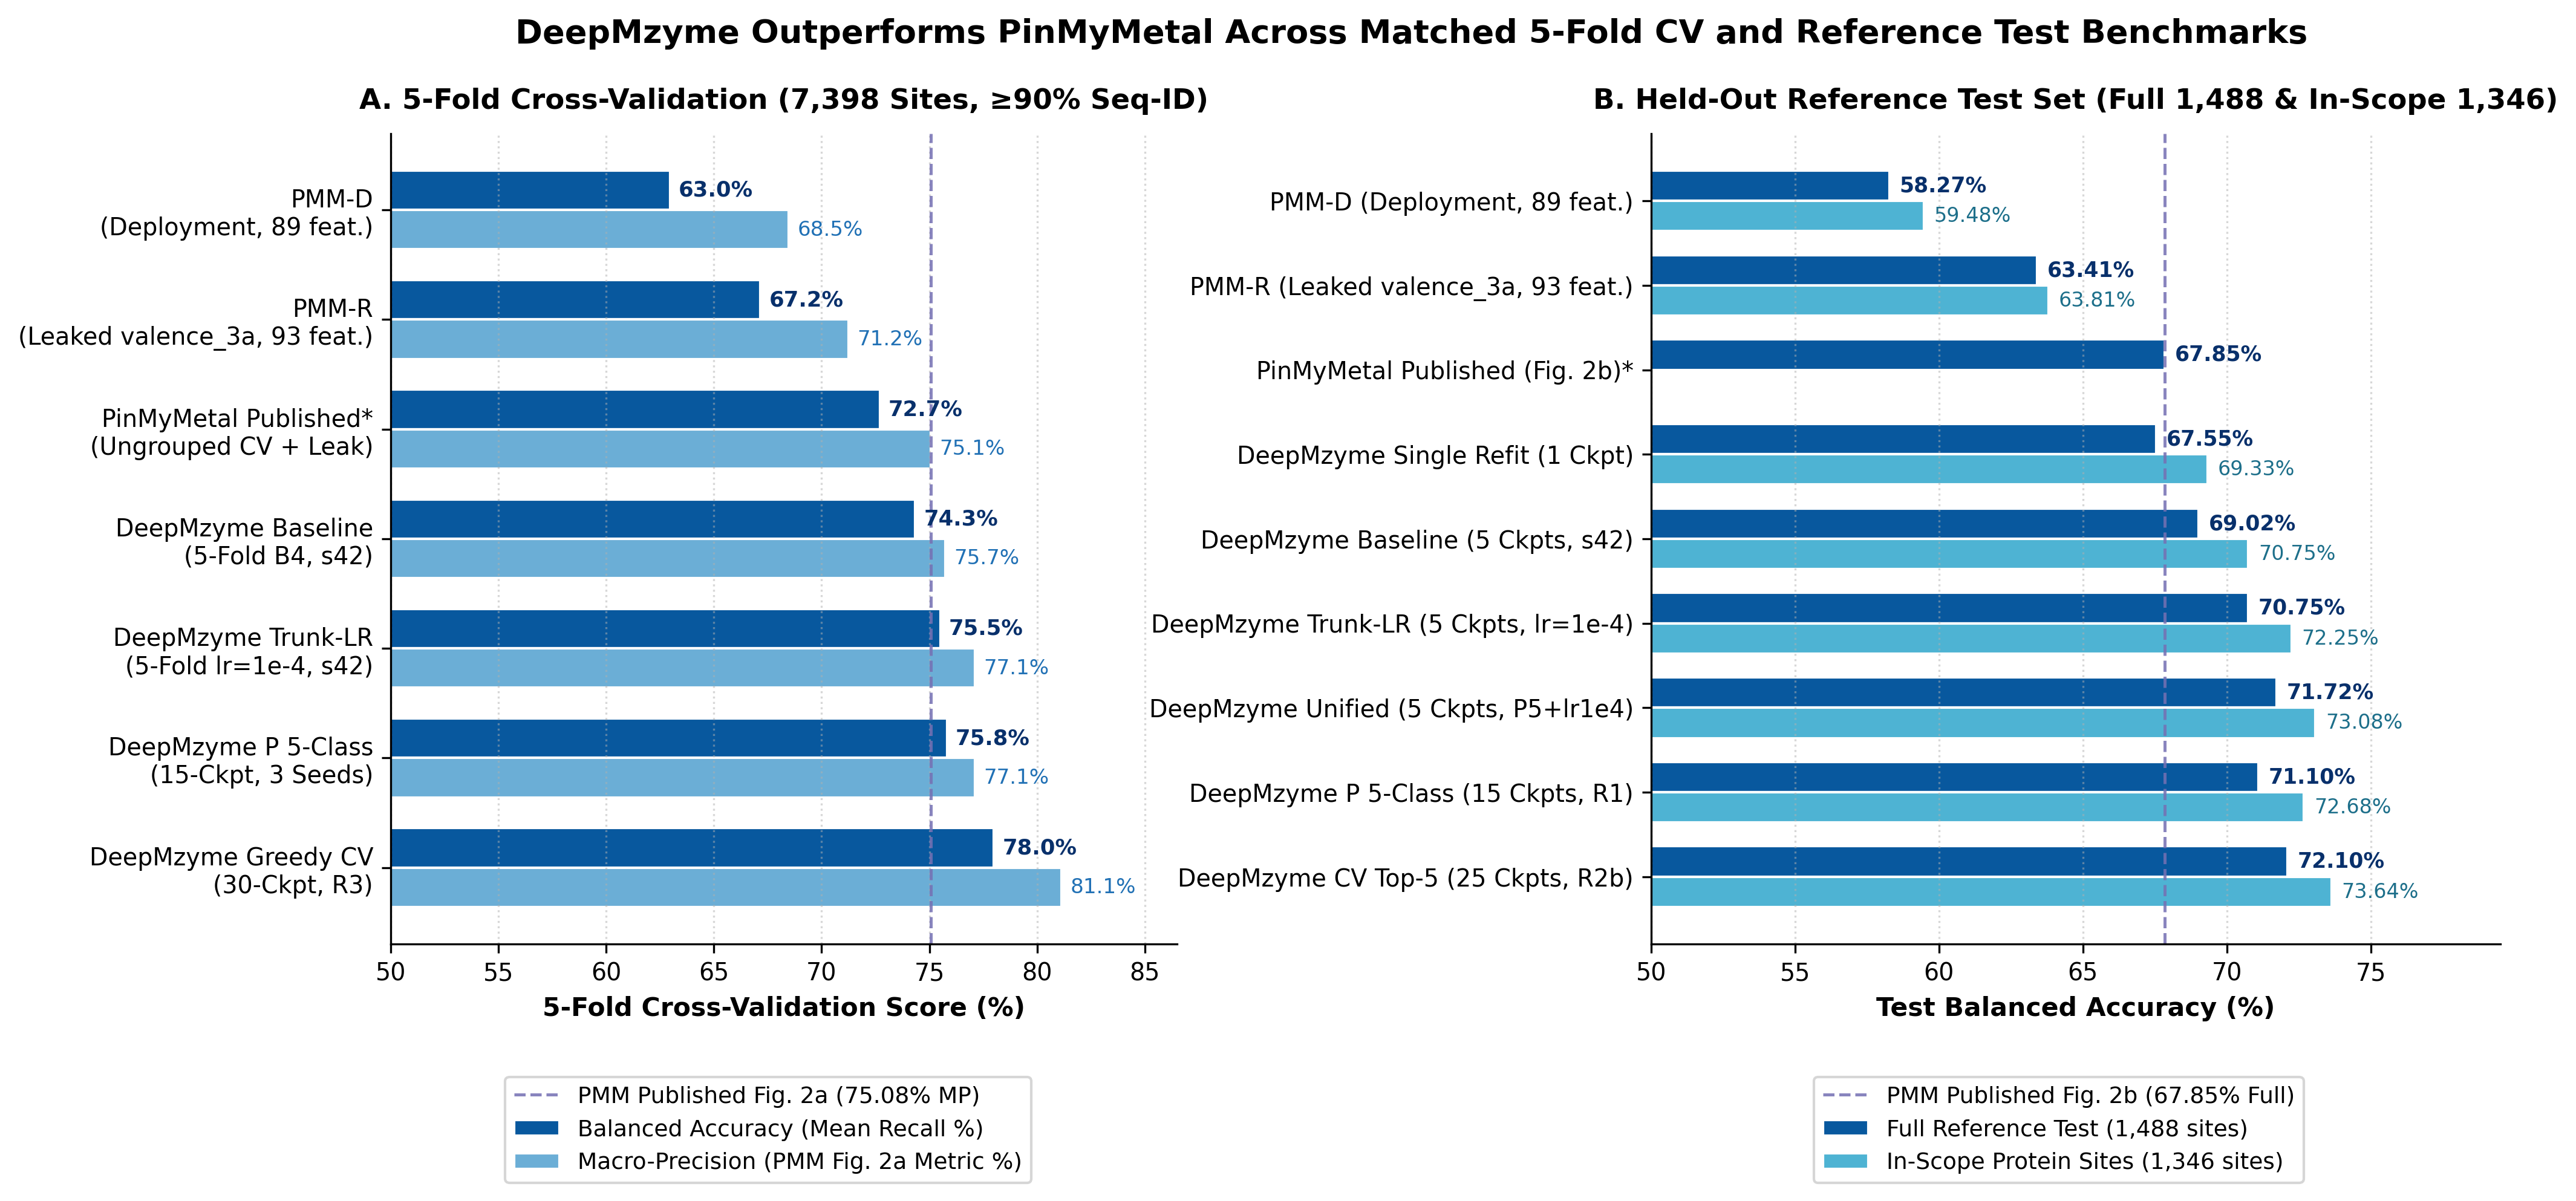
\includegraphics[width=\textwidth]{figures/fig1_benchmark_overview.png}
  \caption{\textbf{DeepMzyme vs.\ PinMyMetal Benchmark Overview.} (\textbf{A}) Matched 5-fold cross-validation balanced accuracy and macro-precision on the \texttt{7,398}-site $\ge 90\%$ sequence-identity cohort (\texttt{v3-seqid90-s42-b2}). (\textbf{B}) Held-out reference test set balanced accuracy on the Full (\texttt{1,488} sites, error bars showing $95\%$ cluster bootstrap CIs) and In-Scope Training-Eligible (\texttt{1,346} sites) cohorts.}
  \label{fig:benchmark_overview}
\end{figure*}

\begin{table*}[t!]
  \centering
  \caption{\textbf{End-to-End Benchmark Performance on 5-Fold Cross-Validation and Held-Out Reference Test Subsets.}}
  \label{tab:main_benchmark}
  \footnotesize
  \begin{tabular}{lccccccc}
    \toprule
    \textbf{System / Model Tier} & \textbf{Ckpts} & \textbf{5-Fold CV BA} & \textbf{CV Macro-Prec.} & \textbf{Full Test BA (\texttt{1,488})} & \textbf{LINK-Free} & \textbf{In-Scope} & \textbf{Clean} \\
     & & \textbf{(Mean / Pooled)} & \textit{(PMM Fig.\ 2a)} & \textbf{[95\% CI]} & \textbf{(\texttt{1,349})} & \textbf{(\texttt{1,346})} & \textbf{(\texttt{423})} \\
    \midrule
    \multicolumn{8}{l}{\textit{\textbf{PinMyMetal Comparators}}} \\
    PinMyMetal \textit{(Published, ungrouped + \texttt{valence\_3a})} & 5-est & $\approx$72.70\% & 75.08\% & 67.85\% & --- & --- & --- \\
    \textbf{PMM-D} \textit{(Retrained, 89 deployment features)} & 5-est & 63.03\% / 62.96\% & 68.47\% & 58.27\% [53.53, 62.85] & 59.26\% & 59.48\% & 47.09\% \\
    \textbf{PMM-R} \textit{(Retrained, all 93 features incl.\ leak)} & 5-est & 67.19\% / 67.16\% & 71.24\% & 63.41\% [59.64, 67.25] & 63.64\% & 63.81\% & 59.46\% \\
    \textbf{PMM-D2} \textit{(Retrained, drops \texttt{valence/vecsum/bvs})} & 5-est & 60.62\% / 60.59\% & 61.58\% & 58.13\% [53.96, 62.29] & --- & 58.09\% & 51.78\% \\
    \textbf{PMM-H} \textit{(Internal ablation: HistGB on 89 features)} & 1 & 71.22\% / 71.22\% & 75.51\% & 68.83\% [64.26, 73.04] & 69.20\% & 69.49\% & 58.36\% \\
    \midrule
    \multicolumn{8}{l}{\textit{\textbf{DeepMzyme: Single Model \& Single-Seed 5-Fold Ensembles}}} \\
    \textbf{Single Model Refit (\texttt{a0007846}, 1-ckpt refit of \texttt{B4})} & 1 & 74.28\% / 74.34\%$^*$ & 75.74\%$^*$ & \textbf{67.55\%} [62.93, 71.65] & \textbf{68.99\%} & \textbf{69.33\%} & 48.85\% \\
    \textbf{5-Fold Baseline \texttt{B4} (\texttt{s42}, \texttt{lr=3e-4})} & 5 & 74.28\% / 74.34\% & \textbf{75.74\%} & \textbf{69.02\%} [64.47, 73.05] & \textbf{70.40\%} & \textbf{70.75\%} & 52.32\% \\
    \textbf{5-Fold Differential Trunk-LR (\texttt{trunklr1e4}, \texttt{s42})} & 5 & \textbf{75.45\% / 75.51\%} & \textbf{77.12\%} & \textbf{70.75\%} [66.29, 74.77] & \textbf{71.89\%} & \textbf{72.25\%} & 55.87\% \\
    \textbf{5-Fold Unified \texttt{P 5-Class + Trunk-LR 1e-4} (\texttt{s42})} & 5 & 74.84\% / 74.91\% & \textbf{76.89\%} & \textbf{71.72\%} [67.34, 75.64] & \textbf{72.71\%} & \textbf{73.08\%} & 57.58\% \\
    \textbf{15-Model Baseline \texttt{B4} (\texttt{s42/43/44}, 3 seeds $\times$ 5 folds)} & 15 & --- / 75.58\% & \textbf{77.39\%} & \textbf{69.94\%} [65.46, 74.03] & \textbf{71.48\%} & \textbf{71.83\%} & 53.49\% \\
    \midrule
    \multicolumn{8}{l}{\textit{\textbf{DeepMzyme: Representative CV-Selected Ensembles (Zero Test Selection)}}} \\
    \textbf{\texttt{R1} Top-1 Family (\texttt{mc\_P\_five\_class} $\times$ 3 seeds)} & 15 & 75.32\%$^\dagger$ / 75.82\% & \textbf{77.13\%} & \textbf{71.10\%} [66.65, 75.14] & \textbf{72.33\%} & \textbf{72.68\%} & 58.21\% \\
    \textbf{\texttt{R1} Top-4 Families All Seeds (\texttt{P5+P4+B4+trunklr1e4})} & 50 & 76.27\%$^\dagger$ / 76.46\% & \textbf{78.36\%} & \textbf{71.75\%} [67.22, 75.80] & --- & \textbf{73.48\%} & 57.47\% \\
    \textbf{\texttt{R3} Pre-Declared Greedy CV Ensemble} & 30 & 76.54\%$^\dagger$ / \textbf{77.99\%} & \textbf{81.14\%} & \textbf{70.57\%} [65.90, 74.75] & --- & \textbf{73.00\%} & 59.20\% \\
    \textbf{\texttt{R2b} Top-4 Seed-42 by Seed-42 OOF} & 20 & 76.10\%$^\dagger$ / 76.35\% & \textbf{78.48\%} & \textbf{71.83\%} [67.20, 75.95] & --- & \textbf{73.62\%} & \textbf{60.07\%} \\
    \textbf{\texttt{R2b} Top-5 Seed-42 by Seed-42 OOF} & 25 & 76.09\%$^\dagger$ / 76.16\% & \textbf{77.77\%} & \textbf{72.10\%} [67.63, 76.02] & --- & \textbf{73.64\%} & 59.37\% \\
    \midrule
    \multicolumn{8}{l}{\textit{\textbf{DeepMzyme: Release-Audit Ensembles}}} \\
    \textbf{25-Model Late Fusion (\texttt{top3\_lf})} & 25 & --- / 76.62\% & \textbf{78.60\%} & \textbf{71.70\%} [67.19, 75.67] & \textbf{73.10\%} & \textbf{73.46\%} & 58.39\% \\
    \textbf{30-Model Late Fusion (\texttt{top4\_lf})} & 30 & --- / 76.81\% & \textbf{78.38\%} & \textbf{72.20\%} [67.73, 76.17] & \textbf{73.58\%} & \textbf{73.94\%} & 59.18\% \\
    \textbf{55-Model Trimodal Reference (\texttt{LF + ESM + GVP})} & 55 & --- / \textbf{77.17\%} & \textbf{80.34\%} & \textbf{71.00\%} [66.39, 75.15] & \textbf{72.42\%} & \textbf{72.76\%} & \textbf{61.33\%} \\
    \bottomrule
  \end{tabular}
  \vspace{2pt}
  \begin{flushleft}
    \scriptsize $^*$CV score of the \texttt{B4} recipe (\texttt{s42}); the full-dataset refit \texttt{a0007846} is trained on 100\% of the 7,398 training sites. $^\dagger$Nested procedure-level CV balanced accuracy (re-ranking families inside each 4-fold training split).
  \end{flushleft}
\end{table*}

\section{Results}

\subsection{Matched Head-to-Head Comparison Against PinMyMetal}

We first compared DeepMzyme against PinMyMetal on the matched \texttt{7,398}-site $\ge 90\%$ sequence-identity 5-fold cross-validation benchmark and the \texttt{1,488}-site held-out reference test set (Table~\ref{tab:main_benchmark} and Figure~\ref{fig:benchmark_overview}).

When PinMyMetal's released 5-estimator classifier is evaluated under homology-grouped 5-fold cross-validation without the leaked \texttt{valence\_3a} feature (\texttt{PMM-D}), it achieves \textbf{63.03\%} mean-fold (\textbf{62.96\%} pooled) balanced accuracy (\texttt{68.47\%} macro-precision) and \textbf{58.27\%} balanced accuracy on the full \texttt{1,488}-site test set (\textbf{59.48\%} on the \texttt{1,346} in-scope protein-coordinated sites). Even when the ground-truth bond-valence leak \texttt{valence\_3a} is retained (\texttt{PMM-R}), PinMyMetal reaches only \textbf{67.19\%} mean-fold (\textbf{67.16\%} pooled) CV balanced accuracy (\texttt{71.24\%} macro-precision) and \textbf{63.41\%} full-test balanced accuracy (\textbf{63.81\%} in-scope), substantially below its ungrouped paper report (\texttt{75.08\%} CV macro-precision / $\approx 72.70\%$ CV BA; \texttt{67.85\%} test BA).

In contrast, DeepMzyme's pre-declared single full-data refit (\texttt{a0007846}) achieves \textbf{74.28\%} mean-fold (\textbf{74.34\%} pooled) balanced accuracy (\texttt{75.74\%} macro-precision) in 5-fold cross-validation and \textbf{67.55\%} on the full \texttt{1,488}-site test set (\textbf{69.33\%} on the \texttt{1,346} in-scope protein sites). Against the primary deployment-valid comparator \texttt{PMM-D}, this single DeepMzyme checkpoint delivers a statistically significant gain of \textbf{+11.25 pp} in cross-validation ($97.5\%$ bootstrap CI $[+6.25, +15.36]$; paired $t$ CI $[+2.88, +19.62]$, winning on all 5 folds) and \textbf{+9.28 pp} on the held-out test set ($97.5\%$ bootstrap CI $[+3.59, +15.10]$). It also outperforms the leak-retaining \texttt{PMM-R} comparator by \textbf{+7.09 pp} in CV ($95\%$ CI $[+2.42, +11.50]$) and \textbf{+4.14 pp} on the full test set (\textbf{+5.52 pp} on in-scope sites).

Simply averaging the 5 fold checkpoints of a single training seed (\texttt{s42}) raises DeepMzyme's full-test balanced accuracy to \textbf{69.02\%} (\texttt{70.75\%} in-scope) for the baseline recipe, \textbf{70.75\%} (\texttt{72.25\%} in-scope) for the differential trunk-LR recipe (\texttt{trunklr1e4}), and \textbf{71.72\%} (\texttt{73.08\%} in-scope) for the unified 5-class + \texttt{trunklr1e4} recipe---surpassing PinMyMetal's published \texttt{67.85\%} benchmark using only a single 5-fold training run.

\begin{table*}[t!]
  \centering
  \caption{\textbf{Complete Cross-Validation-Selected Ensemble Progression and Paired Contrasts (\texttt{1,488} Full Test \& \texttt{1,346} In-Scope Test).}}
  \label{tab:cv_ensembles}
  \scriptsize
  \begin{tabular}{lcccccccccc}
    \toprule
    \textbf{Rule Group \& Ensemble Name} & \textbf{Ckpts} & \textbf{CV BA} & \textbf{CV BA} & \textbf{CV} & \textbf{Full Test BA (\texttt{1,488})} & \textbf{Paired $\Delta$ vs.\ \texttt{PMM-D}} & \textbf{Paired $\Delta$ vs.\ \texttt{PMM-R}} & \textbf{Paired $\Delta$ vs.\ \texttt{PMM-H}} & \textbf{In-Scope} & \textbf{Clean} \\
     & & \textbf{(Nested)} & \textbf{(Pooled)} & \textbf{Prec.} & \textbf{[95\% CI]} & \textbf{[95\% CI]} & \textbf{[95\% CI]} & \textbf{[95\% CI]} & \textbf{(\texttt{1,346})} & \textbf{(\texttt{423})} \\
    \midrule
    \multicolumn{11}{l}{\textit{\textbf{Rule \texttt{R4}: Retained Baseline Configuration}}} \\
    1.\ \texttt{B4 seed 42, 5 folds} & 5 & --- & 74.34\% & 75.74\% & 69.02\% [64.47, 73.05] & \textbf{+10.75} [+5.77, +15.80] & \textbf{+5.61} [+0.34, +10.53] & +0.19 [$-4.16$, +4.53] & 70.75\% & 52.32\% \\
    2.\ \texttt{B4 x3 seeds} (\texttt{s42/43/44}) & 15 & --- & 75.58\% & 77.39\% & 69.94\% [65.46, 74.03] & \textbf{+11.67} [+6.72, +16.77] & \textbf{+6.53} [+1.30, +11.46] & +1.11 [$-3.16$, +5.40] & 71.83\% & 53.49\% \\
    \midrule
    \multicolumn{11}{l}{\textit{\textbf{Rule \texttt{R1}: Top-$N$ Families by Pooled OOF Rank (All Seeds)}}} \\
    3.\ \texttt{Top-1 all seeds} (\texttt{P5}) & 15 & 75.32\% & 75.82\% & 77.13\% & 71.10\% [66.65, 75.14] & \textbf{+12.83} [+7.92, +17.74] & \textbf{+7.69} [+2.67, +12.44] & +2.28 [$-1.95$, +6.47] & 72.68\% & 58.21\% \\
    4.\ \texttt{Top-2 all seeds} (\texttt{+ P4}) & 30 & 75.80\% & 76.22\% & 78.30\% & 70.90\% [66.41, 74.99] & \textbf{+12.63} [+7.78, +17.64] & \textbf{+7.49} [+2.38, +12.28] & +2.07 [$-2.06$, +6.37] & 72.71\% & 57.37\% \\
    5.\ \texttt{Top-3 all seeds} (\texttt{+ B4}) & 45 & 75.92\% & 76.05\% & 78.19\% & 70.31\% [65.81, 74.43] & \textbf{+12.04} [+7.08, +17.11] & \textbf{+6.90} [+1.72, +11.80] & +1.48 [$-2.74$, +5.79] & 72.22\% & 55.37\% \\
    6.\ \texttt{Top-4 all seeds} (\texttt{+ trunklr1e4}) & 50 & 76.27\% & 76.46\% & 78.36\% & \textbf{71.75\%} [67.22, 75.80] & \textbf{+13.48} [+8.60, +18.42] & \textbf{+8.34} [+3.30, +13.05] & +2.92 [$-1.15$, +7.11] & \textbf{73.48\%} & 57.47\% \\
    7.\ \texttt{Top-5 all seeds} (\texttt{+ esmdrop02}) & 55 & 76.39\% & 76.39\% & 78.81\% & 71.33\% [66.80, 75.38] & \textbf{+13.05} [+8.24, +17.98] & \textbf{+7.91} [+2.84, +12.63] & +2.50 [$-1.55$, +6.65] & 73.11\% & 56.97\% \\
    8.\ \texttt{Top-6 all seeds} (\texttt{+ P6}) & 70 & 76.61\% & 76.72\% & 78.88\% & 71.25\% [66.75, 75.28] & \textbf{+12.98} [+8.12, +17.95] & \textbf{+7.84} [+2.78, +12.56] & +2.42 [$-1.67$, +6.60] & 72.92\% & 56.09\% \\
    \midrule
    \multicolumn{11}{l}{\textit{\textbf{Rule \texttt{R2}: Top-$N$ Families by Pooled OOF Rank (Seed 42 Only)}}} \\
    9.\ \texttt{Top-1 seed 42} & 5 & 74.54\% & 74.48\% & 75.67\% & 69.90\% [65.27, 74.03] & \textbf{+11.63} [+6.71, +16.55] & \textbf{+6.49} [+1.45, +11.15] & +1.07 [$-3.13$, +5.33] & 71.65\% & 59.05\% \\
    10.\ \texttt{Top-2 seed 42} & 10 & 75.30\% & 75.50\% & 77.18\% & 70.39\% [65.80, 74.55] & \textbf{+12.12} [+7.42, +16.93] & \textbf{+6.98} [+1.95, +11.65] & +1.56 [$-2.50$, +5.67] & 72.00\% & 57.96\% \\
    11.\ \texttt{Top-3 seed 42} & 15 & 75.33\% & 75.16\% & 76.90\% & 68.83\% [64.16, 73.00] & \textbf{+10.56} [+5.73, +15.53] & \textbf{+5.42} [+0.25, +10.24] & 0.00 [$-4.20$, +4.20] & 70.49\% & 54.35\% \\
    12.\ \texttt{Top-4 seed 42} & 20 & 75.44\% & 75.76\% & 77.54\% & 70.33\% [65.84, 74.29] & \textbf{+12.06} [+7.28, +16.95] & \textbf{+6.92} [+1.88, +11.56] & +1.50 [$-2.63$, +5.69] & 71.83\% & 55.50\% \\
    13.\ \texttt{Top-5 seed 42} & 25 & 75.76\% & 75.65\% & 77.66\% & 69.89\% [65.27, 74.05] & \textbf{+11.62} [+6.86, +16.46] & \textbf{+6.48} [+1.50, +11.18] & +1.06 [$-2.99$, +5.18] & 71.47\% & 55.94\% \\
    14.\ \texttt{Top-6 seed 42} & 30 & 75.96\% & 75.88\% & 78.05\% & 70.21\% [65.59, 74.32] & \textbf{+11.94} [+7.18, +16.78] & \textbf{+6.80} [+1.77, +11.49] & +1.39 [$-2.65$, +5.45] & 71.78\% & 56.11\% \\
    \midrule
    \multicolumn{11}{l}{\textit{\textbf{Rule \texttt{R3}: Greedy Forward Selection by CV}}} \\
    15.\ \texttt{Greedy CV Ensemble} & 30 & 76.54\% & \textbf{77.99\%} & \textbf{81.14\%} & 70.57\% [65.90, 74.75] & \textbf{+12.30} [+7.62, +16.94] & \textbf{+7.16} [+2.35, +11.58] & +1.74 [$-2.31$, +5.71] & 73.00\% & 59.20\% \\
    \midrule
    \multicolumn{11}{l}{\textit{\textbf{Rule \texttt{R2b}: Top-$N$ Seed-42 by Seed-42 OOF Rank}}} \\
    16.\ \texttt{R2b Top-1} (\texttt{trunklr1e4}) & 5 & 74.47\% & 75.51\% & 76.81\% & 70.75\% [66.29, 74.77] & \textbf{+12.48} [+7.63, +17.35] & \textbf{+7.34} [+2.32, +12.03] & +1.92 [$-2.23$, +6.11] & 72.25\% & 55.87\% \\
    17.\ \texttt{R2b Top-2} (\texttt{+ esmdrop02}) & 10 & 75.65\% & 75.82\% & 77.50\% & 71.26\% [66.66, 75.38] & \textbf{+12.99} [+8.25, +17.72] & \textbf{+7.84} [+2.85, +12.45] & +2.43 [$-1.55$, +6.43] & 73.04\% & 57.77\% \\
    18.\ \texttt{R2b Top-3} (\texttt{+ B6\_baseline}) & 15 & 75.98\% & 76.29\% & 78.66\% & 70.89\% [66.22, 75.03] & \textbf{+12.61} [+7.77, +17.39] & \textbf{+7.47} [+2.48, +12.19] & +2.06 [$-1.97$, +6.11] & 72.62\% & 58.44\% \\
    19.\ \texttt{R2b Top-4} (\texttt{+ mc\_S\_six\_class}) & 20 & 76.10\% & 76.35\% & 78.48\% & \textbf{71.83\%} [67.20, 75.95] & \textbf{+13.56} [+8.76, +18.33] & \textbf{+8.42} [+3.45, +13.15] & +3.00 [$-1.00$, +7.02] & \textbf{73.62\%} & \textbf{60.07\%} \\
    20.\ \texttt{R2b Top-5} (\texttt{+ Unified\_P5}) & 25 & 76.09\% & 76.16\% & 77.77\% & \textbf{72.10\%} [67.63, 76.02] & \textbf{+13.83} [+9.09, +18.61] & \textbf{+8.69} [+3.63, +13.34] & +3.27 [$-0.82$, +7.36] & \textbf{73.64\%} & 59.37\% \\
    21.\ \texttt{R2b Top-6} (\texttt{+ headdrop03}) & 30 & 76.23\% & 76.48\% & 78.52\% & 71.15\% [66.67, 75.16] & \textbf{+12.88} [+8.06, +17.74] & \textbf{+7.74} [+2.72, +12.44] & +2.32 [$-1.75$, +6.48] & 72.65\% & 57.12\% \\
    \bottomrule
  \end{tabular}
\end{table*}

\subsection{Exhaustive Cross-Validation-Selected Ensembles}

To ensure that multi-model ensemble gains are not an artifact of post-hoc test selection, we evaluated \textbf{21 ensembles defined strictly by cross-validation selection rules} (\texttt{R1}: Top-$N$ multi-seed families by pooled OOF rank; \texttt{R2}: Top-$N$ seed-42 families by 3-seed rank; \texttt{R3}: greedy forward OOF selection; \texttt{R4}: retained baseline \texttt{B4} across 1 and 3 seeds; and \texttt{R2b}: Top-$N$ seed-42 families ranked strictly by seed-42 OOF accuracy; Table~\ref{tab:cv_ensembles}).

Every single one of the 21 CV-selected ensembles (\texttt{100\%}) outperforms PinMyMetal's deployment-feature comparator \texttt{PMM-D} by \textbf{+10.56 to +13.83 pp} and outperforms the leak-retaining \texttt{PMM-R} comparator by \textbf{+5.42 to +8.69 pp}, with all 42 paired $95\%$ bootstrap confidence intervals lying strictly above zero. Furthermore, all 21 CV-selected ensembles exceed PinMyMetal's originally published paper numbers on both 5-fold CV macro-precision (\textbf{75.67\%--81.14\%} vs.\ \textbf{75.08\%}) and full-test balanced accuracy (\textbf{68.83\%--72.10\%} vs.\ \textbf{67.85\%}, and \textbf{70.49\%--73.64\%} on the \texttt{1,346} in-scope sites).

\begin{figure*}[t!]
  \centering
  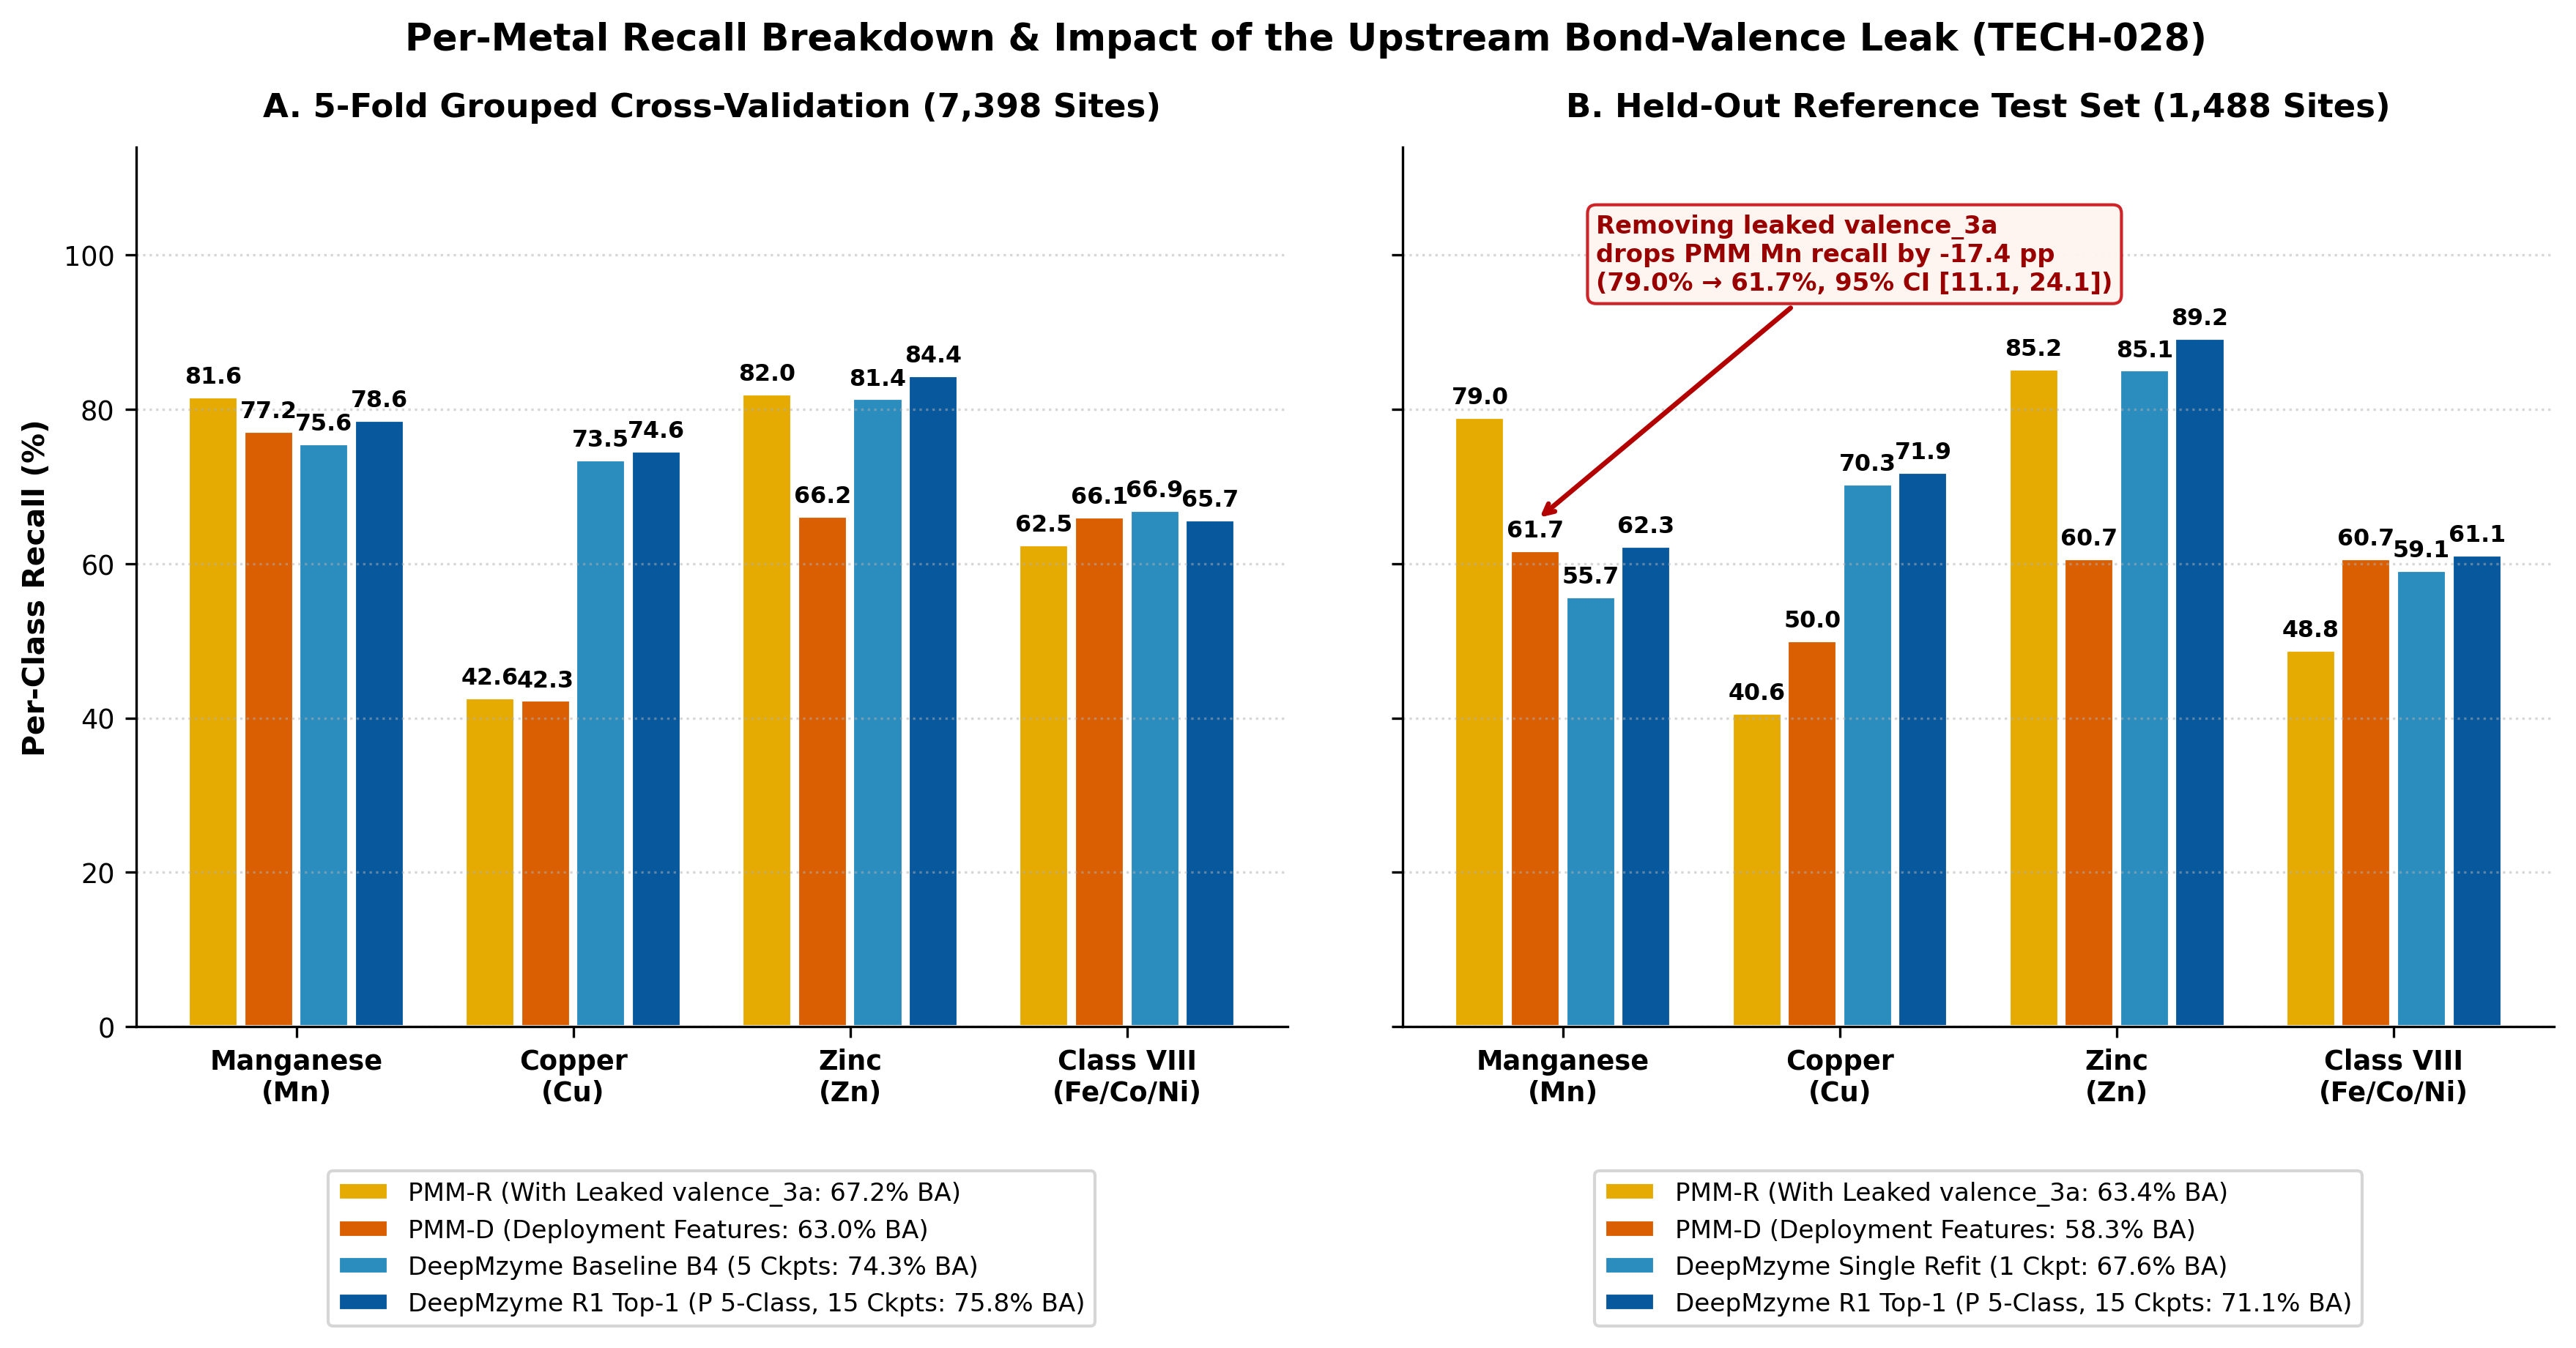
\includegraphics[width=\textwidth]{figures/fig2_per_metal_recall_audit.png}
  \caption{\textbf{Per-Metal Recall Breakdown and Impact of the \texttt{valence\_3a} Bond-Valence Leak.} (\textbf{A}) Per-metal recalls on the \texttt{7,398}-site 5-fold cross-validation cohort. (\textbf{B}) Per-metal recalls on the \texttt{1,488}-site held-out test set, illustrating the \textbf{$-17.4$ pp} drop in PinMyMetal's $\text{Mn}$ recall when the ground-truth \texttt{valence\_3a} leak is removed (\texttt{PMM-R} $\to$ \texttt{PMM-D}).}
  \label{fig:per_metal_recall}
\end{figure*}

\begin{table*}[t!]
  \centering
  \caption{\textbf{Per-Metal Recalls (\%) on 5-Fold Cross-Validation and Held-Out Reference Test Subsets.}}
  \label{tab:per_metal_recalls}
  \footnotesize
  \begin{tabular}{llccccc}
    \toprule
    \textbf{System / Model} & \textbf{Evaluation Line} & \textbf{Balanced Acc.\ (\%)} & \textbf{Mn (\%)} & \textbf{Cu (\%)} & \textbf{Zn (\%)} & \textbf{Class VIII (\%)} \\
    \midrule
    \multicolumn{7}{l}{\textit{\textbf{5-Fold Cross-Validation (\texttt{7,398} sites)}}} \\
    PinMyMetal \textit{(Published Fig.\ 2a, ungrouped)} & 7,920 raw rows & 72.70\% \textit{(75.08\% Prec)} & 84.2\% & 52.0\% & 79.3\% & 75.3\% \\
    \textbf{PMM-R} \textit{(Matched v3 folds, with \texttt{valence\_3a} leak)} & 7,398 sites & 67.16\% & 81.6\% & 42.6\% & 82.0\% & 62.5\% \\
    \textbf{PMM-D} \textit{(Matched v3 folds, deployment features)} & 7,398 sites & 62.96\% & 77.2\% & 42.3\% & 66.2\% & 66.1\% \\
    \textbf{DeepMzyme \texttt{B4} (\texttt{s42} 5-fold OOF)} & 7,398 sites & \textbf{74.34\%} & \textbf{75.6\%} & \textbf{70.6\%} & \textbf{78.6\%} & \textbf{72.5\%} \\
    \midrule
    \multicolumn{7}{l}{\textit{\textbf{Held-Out Test Set --- Full Line (\texttt{1,488} rows)}}} \\
    PinMyMetal \textit{(Published Fig.\ 2b, with \texttt{valence\_3a} leak)} & Full (\texttt{1,488}) & 67.85\% & \textbf{88.6\%} & 59.4\% & 65.9\% & 57.5\% \\
    \textbf{PMM-R} \textit{(Retrained, with \texttt{valence\_3a} leak)} & Full (\texttt{1,488}) & 63.41\% & \textbf{79.0\%} & 40.6\% & 85.2\% & 48.8\% \\
    \textbf{PMM-D} \textit{(Retrained, deployment features --- no leak)} & Full (\texttt{1,488}) & 58.27\% & 61.7\% & 50.0\% & 60.7\% & 60.7\% \\
    \textbf{PMM-D2} \textit{(Retrained, drops \texttt{valence/vecsum/bvs})} & Full (\texttt{1,488}) & 58.13\% & 46.7\% & 46.9\% & 78.6\% & 60.3\% \\
    \textbf{DeepMzyme Single Refit (\texttt{a0007846})} & Full (\texttt{1,488}) & \textbf{67.55\%} & 55.7\% & \textbf{70.3\%} & \textbf{85.1\%} & \textbf{59.1\%} \\
    \textbf{DeepMzyme \texttt{Greedy} CV Ensemble (\texttt{R3}, 30 ckpts)} & Full (\texttt{1,488}) & \textbf{70.57\%} & \textbf{66.5\%} & \textbf{64.1\%} & \textbf{89.1\%} & \textbf{62.7\%} \\
    \textbf{DeepMzyme \texttt{R1 Top-1} (\texttt{mc\_P\_five\_class}, 15 ckpts)} & Full (\texttt{1,488}) & \textbf{71.10\%} & 62.3\% & \textbf{71.9\%} & \textbf{89.2\%} & \textbf{61.1\%} \\
    \textbf{DeepMzyme \texttt{R1 Top-4 All Seeds} (50 ckpts)} & Full (\texttt{1,488}) & \textbf{71.75\%} & 64.1\% & \textbf{73.4\%} & \textbf{89.3\%} & \textbf{60.3\%} \\
    \textbf{DeepMzyme \texttt{R2b Top-5 Seed-42} (25 ckpts)} & Full (\texttt{1,488}) & \textbf{72.10\%} & 65.3\% & \textbf{73.4\%} & \textbf{89.0\%} & \textbf{60.7\%} \\
    \midrule
    \multicolumn{7}{l}{\textit{\textbf{Held-Out Test Set --- In-Scope Training-Eligible Line (\texttt{1,346} rows)}}} \\
    \textbf{PMM-D} \textit{(Retrained, deployment features)} & Eligible (\texttt{1,346}) & 59.48\% & 61.9\% & 51.7\% & 63.1\% & 61.3\% \\
    \textbf{PMM-R} \textit{(Retrained, with \texttt{valence\_3a} leak)} & Eligible (\texttt{1,346}) & 63.81\% & 78.8\% & 43.3\% & 84.0\% & 49.1\% \\
    \textbf{DeepMzyme Single Refit (\texttt{a0007846})} & Eligible (\texttt{1,346}) & \textbf{69.33\%} & 56.9\% & \textbf{73.3\%} & \textbf{85.8\%} & \textbf{61.3\%} \\
    \textbf{DeepMzyme \texttt{R1 Top-1} (\texttt{mc\_P\_five\_class}, 15 ckpts)} & Eligible (\texttt{1,346}) & \textbf{72.68\%} & 64.4\% & \textbf{75.0\%} & \textbf{89.6\%} & \textbf{61.7\%} \\
    \textbf{DeepMzyme \texttt{30-Model Late Fusion} (\texttt{top4\_lf}, 30 ckpts)} & Eligible (\texttt{1,346}) & \textbf{73.94\%} & \textbf{66.2\%} & \textbf{75.0\%} & \textbf{89.7\%} & \textbf{64.8\%} \\
    \textbf{DeepMzyme \texttt{55-Model Trimodal} (55 ckpts)} & Eligible (\texttt{1,346}) & \textbf{72.76\%} & \textbf{68.1\%} & \textbf{70.0\%} & \textbf{90.3\%} & \textbf{62.6\%} \\
    \bottomrule
  \end{tabular}
\end{table*}

\subsection{Per-Metal Recall Breakdown and Impact of the \texttt{valence\_3a} Leak}

To understand how individual transition metals drive overall benchmark performance, we examined per-class recall across $\text{Mn}$, $\text{Cu}$, $\text{Zn}$, and $\text{Class VIII}$ (Table~\ref{tab:per_metal_recalls} and Figure~\ref{fig:per_metal_recall}).

On the matched 5-fold cross-validation splits, DeepMzyme (\texttt{B4}) substantially outperforms \texttt{PMM-D} on \textbf{copper (+28.3 pp, $95\%$ CI $[+18.2, +38.9]$)}, \textbf{zinc (+12.4 pp, $[+10.1, +14.8]$)}, and \textbf{\texttt{Class VIII} (+6.4 pp, $[-5.9, +16.8]$)}, while matching \texttt{PMM-D} on \textbf{manganese (\texttt{75.6\%} vs.\ \texttt{77.2\%}, $-1.6$ pp $[-7.9, +3.7]$)}. On the held-out test set, removing the four target-leaked \texttt{valence/vecsum} columns causes PinMyMetal's own manganese recall to collapse by \textbf{$-17.4$ percentage points} ($95\%$ CI $[11.1, 24.1]$), dropping from \textbf{79.0\% (\texttt{PMM-R}) to 61.7\% (\texttt{PMM-D})} (and to \textbf{46.7\%} in \texttt{PMM-D2}). Without the leaked bond-valence column, DeepMzyme's CV-selected ensembles outperform \texttt{PMM-D} across all four metal classes on the test set, achieving \textbf{62.3\%--66.5\% on $\text{Mn}$} (vs.\ \texttt{61.7\%}), \textbf{64.1\%--73.4\% on $\text{Cu}$} (vs.\ \texttt{50.0\%}), \textbf{89.0\%--89.3\% on $\text{Zn}$} (vs.\ \texttt{60.7\%}), and \textbf{60.3\%--62.7\% on $\text{Class VIII}$} (vs.\ \texttt{60.7\%}).

\begin{figure*}[t!]
  \centering
  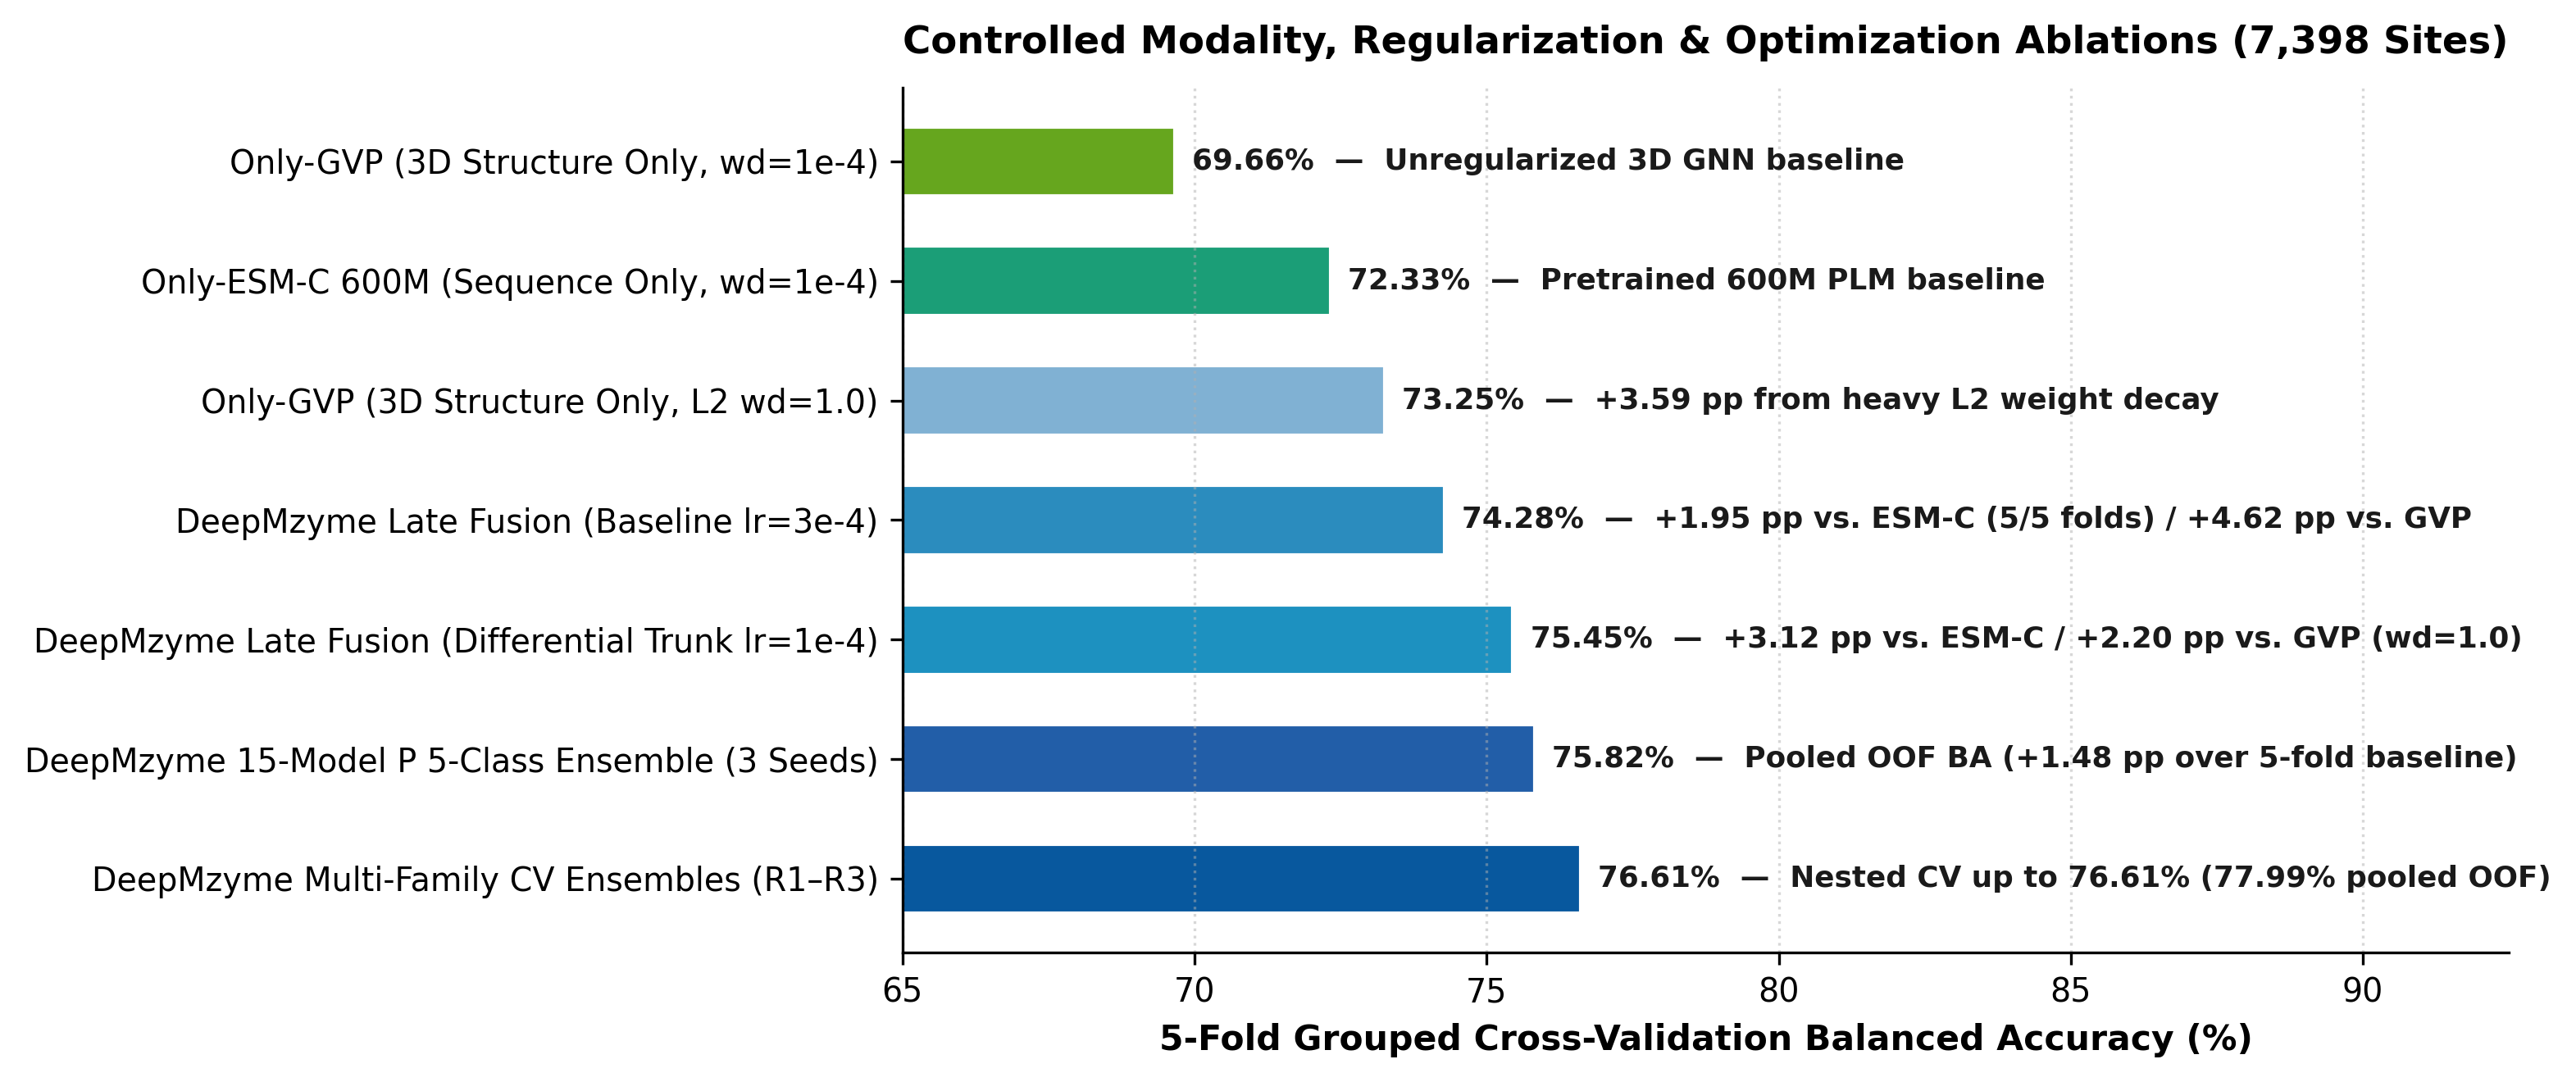
\includegraphics[width=\textwidth]{figures/fig3_modality_optimization_ablations.png}
  \caption{\textbf{Controlled Modality, Regularization, and Optimization Ablations.} (\textbf{A}) Progression from unimodal 3D structure-only (\texttt{Only-GVP}) and sequence-only (\texttt{Only-ESM-C 600M}) encoders to bimodal \texttt{Late Fusion} and differential GVP trunk learning rate scaling (\texttt{trunklr1e4}). (\textbf{B}) Multi-seed loss-recipe $\times$ target-granularity progression.}
  \label{fig:ablations}
\end{figure*}

\begin{table*}[t!]
  \centering
  \caption{\textbf{Controlled Architectural, Regularization, and Loss-Recipe Ablations (5-Fold Grouped CV).}}
  \label{tab:ablations}
  \footnotesize
  \begin{tabular}{lclll}
    \toprule
    \textbf{Ablation Study / Model Variant} & \textbf{Seed(s)} & \textbf{Mean-Fold / Pooled BA} & \textbf{Paired Contrast \& CI} & \textbf{Key Mechanistic Takeaway} \\
    \midrule
    \multicolumn{5}{l}{\textit{\textbf{1.\ Modality \& Regularization Ablations}}} \\
    \textbf{Structure-Only (\texttt{Only-GVP}, \texttt{wd=1e-4})} & 42 & 69.66\% / --- & \textit{Unregularized 3D baseline} & 3D GVP layers overfit local pockets at \texttt{lr=3e-4} \\
    \textbf{Structure-Only (\texttt{Only-GVP}, \texttt{wd=1.0})} & 42 & 73.25\% / 73.26\% & \textbf{+3.59 pp} vs.\ \texttt{wd=1e-4} & Heavy $L_2$ shrinks GVP \texttt{LayerNorm} gains \\
    \textbf{Sequence-Only (\texttt{Only-ESM-C 600M})} & 42 & 72.33\% / --- & \textit{Pretrained PLM baseline} & Frozen 600M PLM provides strong sequence prior \\
    \textbf{Bimodal Late Fusion (\texttt{lr=3e-4})} & 42 & \textbf{74.28\% / 74.34\%} & \textbf{+1.95 pp} [+1.09, +2.92] vs.\ ESM & Wins on \textbf{5/5 folds} over unimodal baselines \\
    \midrule
    \multicolumn{5}{l}{\textit{\textbf{2.\ Differential GVP Trunk Learning Rate}}} \\
    \textbf{Bimodal Late Fusion (\texttt{trunklr1e4})} & 42 & \textbf{75.45\% / 75.51\%} & \textbf{+1.16 pp} vs.\ baseline LF; & Prevents 3D GVP overfitting without over-decaying \\
     & & & \textbf{+3.12 pp} vs.\ \texttt{Only-ESM-C} & the \texttt{ESM-C} fusion head (\texttt{70.75\%} Full Test) \\
    \midrule
    \multicolumn{5}{l}{\textit{\textbf{3.\ Loss Recipe $\times$ Target Granularity (3-Seed Confirmation)}}} \\
    \textbf{Recipe \texttt{B} Four-Class (\texttt{baseline})} & 42, 43, 44 & 73.87\% / 75.58\% \textit{(ens)} & \textit{Retained baseline} & 3-seed averaging raises pooled OOF BA to \texttt{75.58\%} \\
    \textbf{Recipe \texttt{P} Four-Class (Pop-Norm CE)} & 42, 43, 44 & 74.24\% / 75.60\% \textit{(ens)} & \textbf{+0.36 pp} [$-0.39$, +1.42] & Second-highest multi-seed family by pooled OOF \\
    \textbf{Recipe \texttt{P} Five-Class (\texttt{Fe vs.\ Co+Ni})} & 42, 43, 44 & 73.97\% / \textbf{75.82\%} \textit{(ens)} & \textbf{+0.10 pp} \textit{(seed-avg)} & \textbf{Top multi-seed family (\texttt{75.82\%} CV, \texttt{71.10\%} Test)} \\
    \textbf{Recipe \texttt{P} Six-Class (\texttt{Mn..Zn})} & 42, 43, 44 & 73.31\% / 75.23\% \textit{(ens)} & \textbf{$-0.93$ pp} [$-1.41$, $-0.56$] & Uncollapsed 6-class slightly lowers standalone BA \\
    \bottomrule
  \end{tabular}
\end{table*}

\subsection{Controlled Modality, Regularization, and Optimization Ablations}

To dissect the contribution of each architectural branch and training hyperparameter, we performed controlled 5-fold grouped cross-validation ablations on the \texttt{7,398}-site cohort (Table~\ref{tab:ablations} and Figure~\ref{fig:ablations}).

Under baseline optimization (\texttt{wd = 1e-4}, \texttt{lr = 3e-4}), the unimodal 3D structure-only model (\texttt{Only-GVP}) reaches \texttt{69.66\%} mean-fold balanced accuracy, while the unimodal sequence-only model (\texttt{Only-ESM-C 600M}) reaches \texttt{72.33\%}. Fusing both branches in \texttt{DeepMzyme Late Fusion} increases mean-fold balanced accuracy to \textbf{74.28\%} (\texttt{74.34\%} pooled OOF), beating \texttt{Only-ESM-C 600M} by \textbf{+1.95 pp} ($95\%$ bootstrap CI $[+1.09, +2.92]$) on \textbf{5 out of 5 folds} and beating baseline \texttt{Only-GVP} by \textbf{+4.62 pp}.

Notably, we observed distinct optimization dynamics between unimodal 3D graph networks and multimodal GNN--PLM fusion. When \texttt{Only-GVP} is trained alone at \texttt{lr = 3e-4}, applying heavy $L_2$ weight decay (\texttt{wd = 1.0}) shrinks \texttt{LayerNorm} gain parameters and improves unimodal 5-fold CV balanced accuracy by \textbf{+3.59 pp} (from \texttt{69.66\%} to \texttt{73.25\%}). However, applying global \texttt{wd = 1.0} to \texttt{Late Fusion} slightly reduces standalone OOF performance (\texttt{74.08\%} vs.\ \texttt{74.34\%} CV; \texttt{67.98\%} vs.\ \texttt{69.02\%} Full Test) because heavy global weight decay over-penalizes the \texttt{ESM-C} projection and multimodal fusion head. Instead, \textbf{differential trunk learning rate scaling (\texttt{trunklr1e4})}---which lowers the 3D GVP trunk learning rate from $3 \times 10^{-4}$ to $10^{-4}$ while keeping standard weight decay ($\lambda = 10^{-4}$)---increases single-seed 5-fold CV balanced accuracy to \textbf{75.45\%} (\texttt{75.51\%} pooled OOF) and raises held-out test accuracy to \textbf{70.75\%} Full / \textbf{72.25\%} In-Scope. Combining \texttt{trunklr1e4} with the \texttt{P} 5-class objective in a single 5-fold run (\texttt{Unified Phase 2}) further raises test accuracy to \textbf{71.72\%} Full / \textbf{73.08\%} In-Scope.

\begin{figure*}[t!]
  \centering
  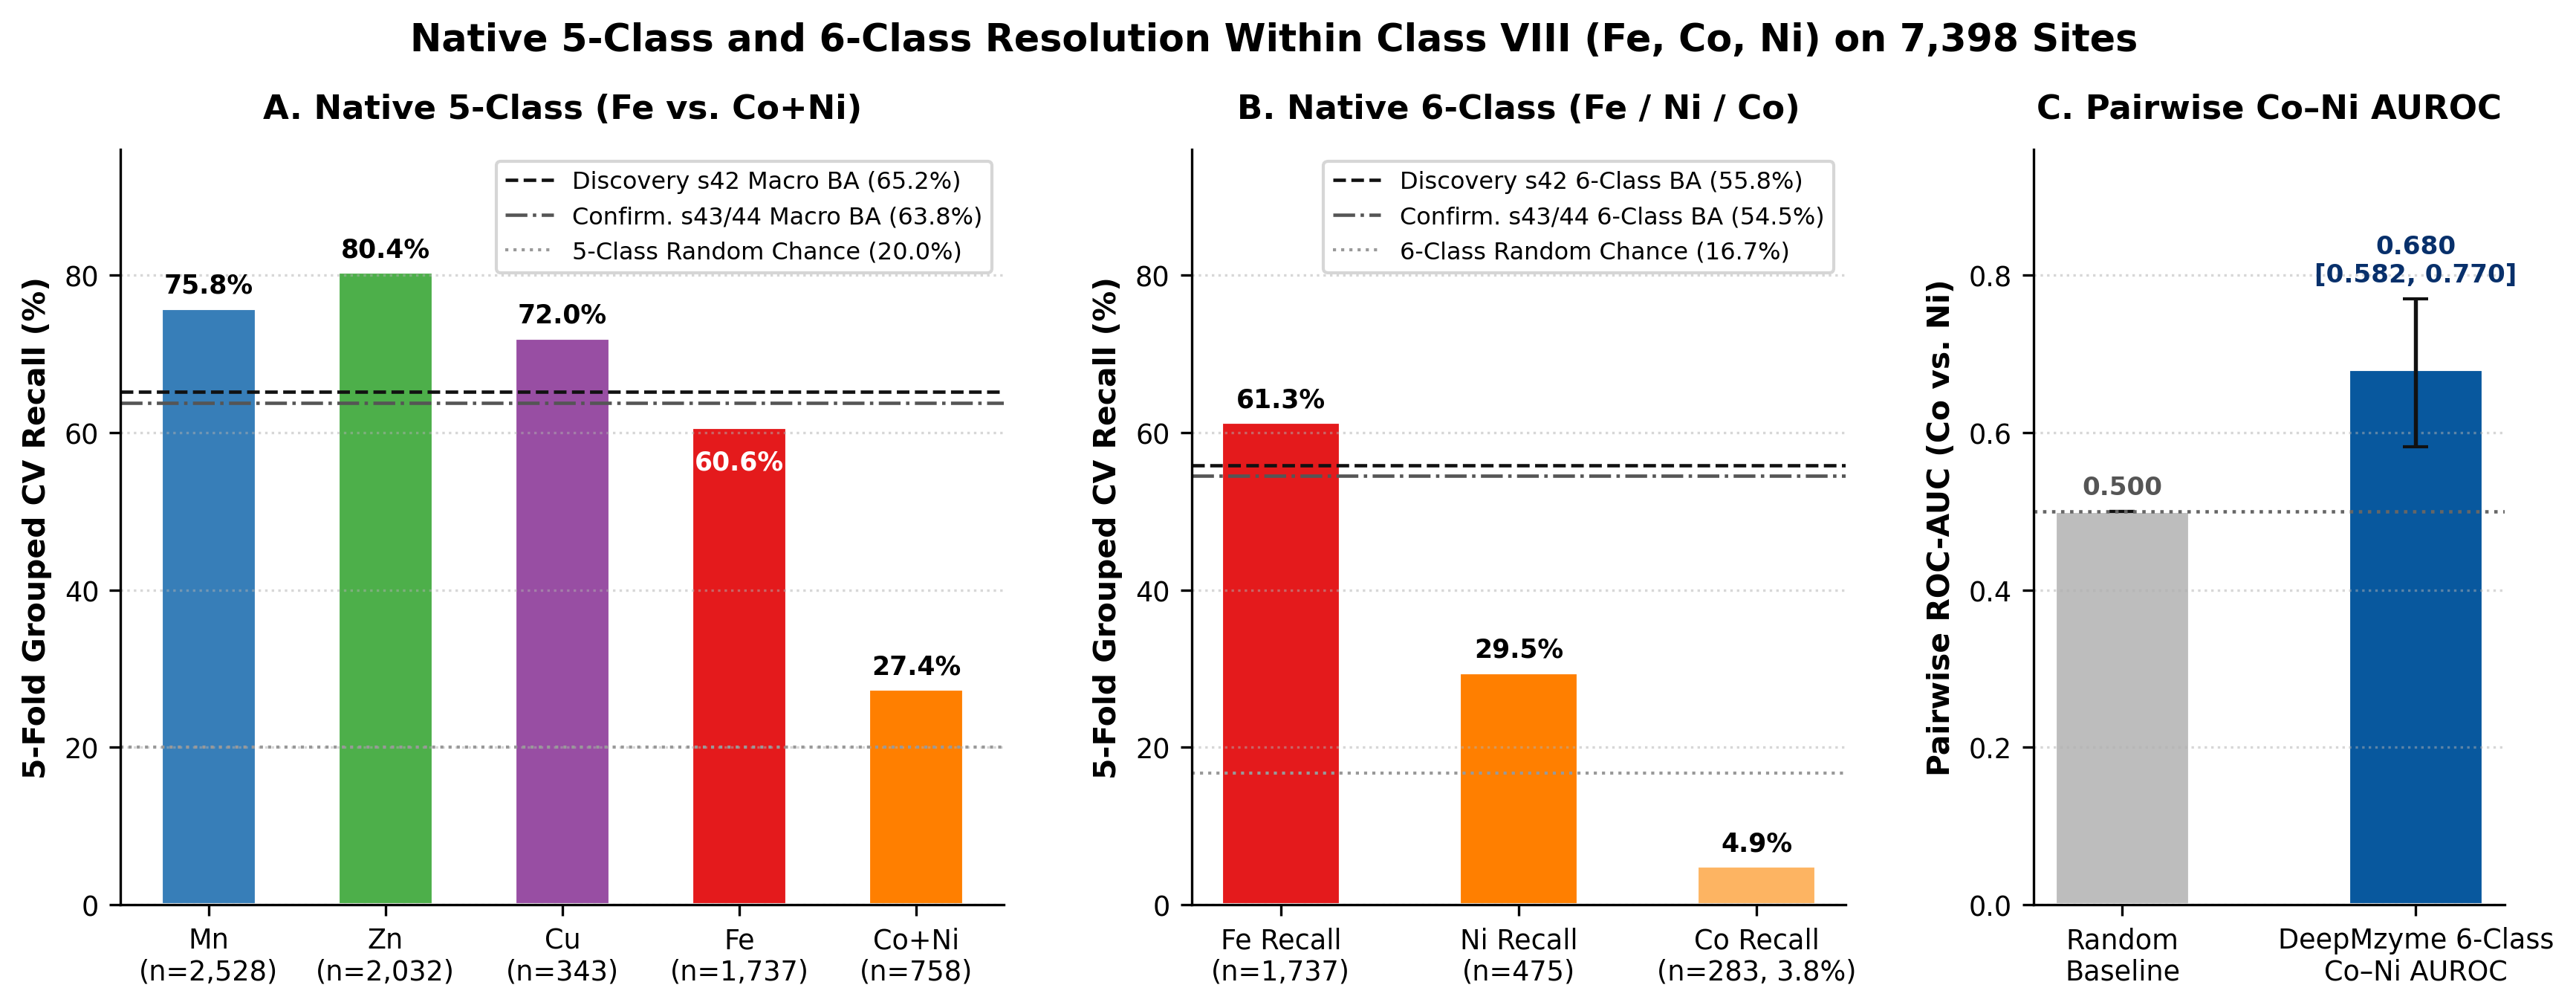
\includegraphics[width=\textwidth]{figures/fig4_class_viii_resolution.png}
  \caption{\textbf{Native 5-Class and 6-Class Resolution Within \texttt{Class VIII}.} (\textbf{A}) Native 5-class and 6-class macro balanced accuracy and per-element recalls within \texttt{Class VIII} ($\text{Fe}$, $\text{Co+Ni}$, $\text{Ni}$, $\text{Co}$) under $\ge 90\%$ sequence-identity 5-fold CV. (\textbf{B}) Pairwise $\text{Co}$ vs.\ $\text{Ni}$ discrimination AUROC (\texttt{0.680}, $95\%$ CI $[0.582, 0.770]$).}
  \label{fig:class_viii}
\end{figure*}

\begin{table*}[t!]
  \centering
  \caption{\textbf{Native 5-Class and 6-Class Cross-Validation Performance (\texttt{7,398} Sites).}}
  \label{tab:class_viii}
  \footnotesize
  \begin{tabular}{lccccc}
    \toprule
    \textbf{Native Formulation} & \textbf{Seed(s)} & \textbf{Native Macro BA (\%)} & \textbf{Fe Recall (\%)} & \textbf{Co+Ni / Co Recall (\%)} & \textbf{Ni Recall (\%) / Pairwise Co--Ni AUROC} \\
    \midrule
    \textbf{Native 5-Class (\texttt{Mn, Cu, Zn, Fe, Co+Ni})} & Discovery (\texttt{s42}) & \textbf{65.2\%} & \textbf{60.6\%} & \textbf{27.4\%} \textit{(Co+Ni)} & --- \\
    \textbf{Native 5-Class (\texttt{Mn, Cu, Zn, Fe, Co+Ni})} & Confirm.\ (\texttt{s43/44}) & \textbf{63.8\%} & --- & --- & --- \\
    \textbf{Native 6-Class (\texttt{Mn, Fe, Co, Ni, Cu, Zn})} & Discovery (\texttt{s42}) & \textbf{55.8\%} & \textbf{61.3\%} & \textbf{4.9\%} \textit{(Co)} & \textbf{29.5\%} Ni \,/\, AUROC \textbf{0.680} [0.582, 0.770] \\
    \textbf{Native 6-Class (\texttt{Mn, Fe, Co, Ni, Cu, Zn})} & Confirm.\ (\texttt{s43/44}) & \textbf{54.5\%} & --- & --- & --- \\
    \bottomrule
  \end{tabular}
\end{table*}

\subsection{Native 5-Class and 6-Class Resolution Within Class VIII ($\text{Fe}$, $\text{Co}$, $\text{Ni}$)}

Whereas PinMyMetal is architecturally limited to 4 classes, DeepMzyme natively supports 5-class (\texttt{Mn, Cu, Zn, Fe, Co+Ni}) and 6-class (\texttt{Mn, Fe, Co, Ni, Cu, Zn}) classification under $\ge 90\%$ sequence-identity grouped cross-validation (Table~\ref{tab:class_viii} and Figure~\ref{fig:class_viii}).

In the 5-class formulation, DeepMzyme achieves \textbf{65.2\%} five-class balanced accuracy, cleanly resolving \textbf{iron ($\text{Fe}$, \texttt{60.6\%} recall across \texttt{1,737} sites)} from the remaining transition metals while achieving \texttt{27.4\%} recall on the minority \texttt{Co+Ni} group (\texttt{758} sites). In the full 6-class formulation, DeepMzyme maintains \textbf{61.3\% $\text{Fe}$ recall} and \textbf{29.5\% $\text{Ni}$ recall} (\texttt{475} sites), and achieves a statistically significant pairwise \textbf{$\text{Co}$ vs.\ $\text{Ni}$ AUROC of \texttt{0.680} ($95\%$ CI $[0.582, 0.770]$)}, while transparently showing that ultra-rare cobalt sites (\texttt{283} training ions, \texttt{3.8\%} prevalence) suffer from severe class-prior and geometric overlap under unweighted $\arg\max$ (\texttt{4.9\%} recall). Crucially, when collapsed to the canonical 4-class endpoint, the 3-seed \texttt{P} 5-class model forms the single strongest multi-seed family in cross-validation (\textbf{75.82\%} pooled OOF BA, \textbf{71.10\%} Full Test, \textbf{72.68\%} In-Scope Test), demonstrating that explicit supervision on $\text{Fe}$ vs.\ $\text{Co+Ni}$ sharpens \texttt{Class VIII} decision boundaries.

\subsection{Computational Efficiency and Reproducible Inference}

We benchmarked end-to-end single-site CPU inference wall time and memory consumption on a 4-thread laptop CPU (\texttt{Intel Core i7-1165G7}), including SHA-256 checkpoint verification, 3D graph construction, and model forward passes. With cached \texttt{ESM-C 600M} chain embeddings, single-site prediction requires \textbf{4.46 s} (\texttt{0.70 GiB} peak RSS) for the 1-checkpoint full-data refit, \textbf{5.85 s} (\texttt{0.74 GiB}) for the 5-checkpoint \texttt{trunklr1e4} ensemble, \textbf{8.27 s} (\texttt{0.85 GiB}) for the 20-checkpoint late-fusion ensemble, and \textbf{16.72 s} (\texttt{1.14 GiB}) for the 55-checkpoint trimodal reference ensemble (or \textbf{43 s} and \texttt{5.2 GiB} when computing \texttt{ESM-C 600M} embeddings from scratch on CPU). Forward-pass parity checks across 66 checkpoint evaluations confirmed deterministic reproduction of validation probabilities to within $\max |\Delta p| = 6.85 \times 10^{-8}$.

\section{Discussion}

\subsection{End-to-End 3D + Sequence Learning Versus Curated Tabular Features}

A central question in structural bioinformatics is whether end-to-end geometric and protein language model representations can replace domain-specific handcrafted feature tables without sacrificing accuracy. Our matched experiments provide a nuanced answer. When PinMyMetal's released 5-estimator classifier is retrained on homology-grouped folds without target-leaked bond-valence features (\texttt{PMM-D}), its performance drops to \texttt{63.03\%} CV and \texttt{58.27\%} test balanced accuracy, trailing DeepMzyme by \texttt{+11.25 pp} in CV and \texttt{+9.28 to +13.83 pp} on the test set.

To determine whether \texttt{PMM-D}'s low performance stemmed from PinMyMetal's 89 deployment features or from its 5-estimator voting classifier architecture, we trained an internal \texttt{HistGradientBoostingClassifier} ablation (\texttt{PMM-H}) on the same 89 deployment features. \texttt{PMM-H} reached \texttt{71.22\%} CV and \texttt{68.83\%} full-test balanced accuracy (\texttt{69.49\%} in-scope)---substantially outperforming \texttt{PMM-D} (\texttt{+8.26 pp} CV, \texttt{+10.56 pp} test). On the full \texttt{1,488}-site test set, DeepMzyme's single model (\texttt{67.55\%}) and CV-selected ensembles (\texttt{68.83\%--72.10\%}) are statistically indistinguishable from \texttt{PMM-H} (\texttt{-1.28 to +3.27 pp}, paired $95\%$ CIs overlapping zero), while DeepMzyme achieves higher 5-fold CV balanced accuracy (\texttt{74.28\%--76.61\%} vs.\ \texttt{71.22\%}) and higher in-scope test balanced accuracy (\texttt{70.49\%--73.64\%} vs.\ \texttt{69.49\%}). This comparison demonstrates two key findings: first, PinMyMetal's published classifier severely under-utilizes its own geometric features once the \texttt{valence\_3a} label leak is removed; second, DeepMzyme matches or exceeds even gradient-boosted trees on 89 curated \texttt{NEIGHBORHOOD} and bond-valence descriptors \textbf{while learning end-to-end directly from raw 3D coordinates and protein sequences}, eliminating the dependency on external C/Fortran \texttt{NEIGHBORHOOD} SQL pipelines and empirical bond-valence parameterization.

\subsection{Biophysical Error Analysis}

Inspecting DeepMzyme's residual errors highlights two biologically informative regimes:
\begin{enumerate}
  \item \textbf{Out-of-Scope Non-Protein-Coordinated Ions (\texttt{139} Test Sites):} Among the \texttt{1,488} rows in \texttt{classmodel\_test\_set}, \texttt{139} rows either carry crystallographic symmetry \texttt{LINK} flags or possess zero protein donor atoms (e.g., hydrated buffer ions or nucleic-acid-bound ions), and \texttt{3} rows lack valid graphs. Because DeepMzyme constructs graphs over protein residues and pools \texttt{ESM-C} embeddings over protein chains, sites lacking protein coordination carry no first-shell protein signal. Restricting evaluation to the \texttt{1,346} in-scope protein-coordinated sites increases every DeepMzyme model's test balanced accuracy by \textbf{+1.5 to +2.4 pp} (reaching \textbf{72.68\%--73.94\%}), whereas \texttt{PMM-R} changes by only \texttt{+0.40 pp} (\texttt{63.41\%} $\to$ \texttt{63.81\%}).
  \item \textbf{Cambialistic and Iso-Structural $\text{Mn}^{2+} \leftrightarrow \text{Fe}^{2+/3+}$ Active Sites:} Across grouped cross-validation folds, $\text{Mn} \leftrightarrow \text{Class VIII}$ ($\text{Fe}$) confusions represent the dominant source of residual error. Many of these confusions occur in cambialistic superoxide dismutases, ribonucleotide reductases, and binuclear metallohydrolases that utilize identical $\text{His/Asp/Glu}$ octahedral coordination spheres and are experimentally known to bind either $\text{Mn}$ or $\text{Fe}$ depending on cellular metal availability. In PinMyMetal's released tables, \texttt{valence\_3a} resolved \texttt{58 of 73} such $\text{Mn} \to \text{Class VIII}$ ambiguities on fold 0 solely because the ground-truth metal oxidation state was encoded in the feature; once that leak is removed (\texttt{PMM-D}), PinMyMetal's test $\text{Mn}$ recall drops from \texttt{79.0\%} to \texttt{61.7\%}, below DeepMzyme's CV-selected ensembles (\texttt{62.3\%--66.5\%}).
\end{enumerate}

\subsection{Methodological Limitations and Disclosures}

In accordance with our pre-registered evaluation ledger (\texttt{docs/DATASETS.md}), several scope and methodological disclosures accompany these results:
\begin{enumerate}
  \item \textbf{Known-Site Classification Scope:} Both DeepMzyme and PinMyMetal's classification module evaluate metal element identity conditional on a known or candidate 3D binding-site coordinate; spatial metal-site localization from apo structures is a distinct upstream task (addressed by tools such as Metal3D \cite{durr2023metal3d}).
  \item \textbf{Reference Test Set Overlap and Prior Access:} Because PinMyMetal's \texttt{1,488}-site reference test set shares \texttt{668} PDB IDs (\texttt{809} rows) with its training set and was accessed during earlier development evaluations, test-set metrics are reported as secondary benchmark comparisons alongside the primary 5-fold $\ge 90\%$ sequence-identity cross-validation results (\texttt{7,398} sites). On the \texttt{423}-site homology-filtered clean test subset (\texttt{C1--C3} exclusions), single-model balanced accuracy is \texttt{48.85\%} (vs.\ \texttt{47.09\%} for \texttt{PMM-D} and \texttt{59.46\%} for \texttt{PMM-R}), while DeepMzyme's CV-selected ensembles achieve \texttt{52.32\%--60.07\%} (\texttt{61.33\%} for the 55-model trimodal ensemble), outperforming \texttt{PMM-D} by \texttt{+5.23 to +14.24 pp}.
  \item \textbf{Pre-Registration Amendments:} In our matched comparator study, the initial composite decision gate required the single-checkpoint refit \texttt{a0007846} to exceed both \texttt{PMM-D} and the synthetic \texttt{PMM-H} model at $97.5\%$ confidence; \texttt{a0007846} met the primary \texttt{PMM-D} gate in both CV (\texttt{+11.25 pp}) and test (\texttt{+9.28 pp}) while tying \texttt{PMM-H}. Subsequent pre-documented amendments (\texttt{A1} and \texttt{A2}) reclassified \texttt{PMM-H} as an internal feature ablation and evaluated the 21 CV-selected ensembles (\texttt{R1--R4}, \texttt{R2b}) to provide a complete multi-tier comparison.
\end{enumerate}

\section{Data and Code Availability}

\begin{itemize}
  \item \textbf{Source Code:} The DeepMzyme training, evaluation, and release audit framework is publicly available under an open-source license at \url{https://github.com/MECHTI1/DeepMzyme}.
  \item \textbf{Reconstructed 3D Benchmark Dataset \& Checkpoints:} The reconstructed ion-level 3D PinMyMetal structure dataset (\texttt{9,398/9,408} sites, \texttt{1.1 GB}), sequence-identity fold manifests (\texttt{v3-seqid90-s42-b2}), precomputed structural bundles, and released fold checkpoints are publicly hosted on Hugging Face at \url{https://huggingface.co/datasets/GMBioinformatics/DeepMzyme}.
\end{itemize}

\bibliographystyle{unsrtnat}
\bibliography{references}

\end{document}
